\documentclass[conference]{IEEEtran}
\IEEEoverridecommandlockouts
% The preceding line is only needed to identify funding in the first footnote. If that is unneeded, please comment it out.
\usepackage[numbers]{natbib}
\usepackage{amsmath,amssymb,amsfonts}
\usepackage{algorithmic}
\usepackage{subcaption}
\usepackage{graphicx}
\usepackage{textcomp}
\usepackage{xcolor}
\def\BibTeX{{\rm B\kern-.05em{\sc i\kern-.025em b}\kern-.08em
    T\kern-.1667em\lower.7ex\hbox{E}\kern-.125emX}}
\begin{document}

%\title{Availability Evaluation Models for Unmanned Aerial Vehicles (UAVs): One Analytical and One Numerical Method\\
\title{Availability Evaluation of Unmanned Aerial Vehicles (UAVs): An Approach Adopting Analytical and Numerical Methods\\

\thanks{}
}

\author{
  \IEEEauthorblockN{Luan Lins\IEEEauthorrefmark{1}, Paulo Maciel\IEEEauthorrefmark{1}, Jamilson Dantas\IEEEauthorrefmark{1}, Jean Araujo\IEEEauthorrefmark{2}, Jeongseok Hyun, Minseok Jang, Kwonsu Jeon, Tuan Anh Nguyen, Jae-Woo Lee*
   }
    \IEEEauthorblockA{\IEEEauthorrefmark{1}Centro de Informática, Universidade Federal de Pernambuco, Recife, Brazil \\}
    \IEEEauthorblockA{\IEEEauthorrefmark{2}Universidade Federal do Agreste de Pernambuco, Garanhuns, Brazil \\}
    \{lcsl2, prmm, jrd\}@cin.ufpe.br, jean.teixeira@ufape.edu.br
}

%\author{
%\IEEEauthorblockN{1\textsuperscript{st} Luan Lins}
%\IEEEauthorblockA{\textit{Centro de Informática} \\
%\textit{Universidade Federal de Pernambuco}\\
%Recife-PE, Brazil \\
%lcsl2@cin.ufpe.br}
%\and
%\IEEEauthorblockN{ Paulo Maciel}
%\IEEEauthorblockA{\textit{Centro de Informática} \\
%\textit{Universidade Federal de Pernambuco}\\
%Recife-PE, Brazil \\
%prrm@cin.ufpe.br}
%\and
%\IEEEauthorblockN{ Jamilson Dantas}
%\IEEEauthorblockA{\textit{Centro de Informática} \\
%\textit{Universidade Federal de Pernambuco}\\
%Recife-PE, Brazil \\
%jrd@cin.ufpe.br}
%\and
%\IEEEauthorblockN{ Jean Araujo}
%\IEEEauthorblockA{\textit{Universidade Federal do Agreste de Pernambuco}\\
%Recife-PE, Brazil \\
%teixeirajean1@gmail.com}

%}

\maketitle

\begin{abstract}
%The reliability and availability evaluation of unmanned aerial vehicles (UAVs) is essential, especially when these are used to save lives. However, the infrastructure planning of the UAVs is not an easy task. Thus, the hierarchical modeling strategy may guide designers to evaluate and compare some results with already implemented proposals. This paper proposes a methodology and models to evaluate the availability of critical systems implemented in unmanned aerial vehicles. Two models are proposed: The first is an analytical model to evaluate availability metrics in the primary operating mode. The second model is a numerical method model with Petri nets to use redundancy mechanisms when improving the primary operational mode no longer has as much impact. The validation of the models takes place by comparing the results obtained with the system using different scenarios. In this work, we present three case studies showing the use of the suggested technique to evaluate a UAV flight system, given the improvements and models used. The results show that it is possible to have an availability increase of 164.71\% in each technique and 193.82\% in mixed-use.

The availability evaluation of unmanned aerial vehicles (UAVs) is essential, especially when they are used to save lives. However, infrastructure planning of UAVs is challenging since they have small components and limited usable time. This paper proposes a methodology and models based on stochastic Petri nets and Markov chains to evaluate the availability of critical systems implemented in unmanned aerial vehicles. As these UAVs follow basic systems with one running drone and one spare drone, the hierarchical modeling strategy may guide designers in evaluating and comparing results with already implemented proposals. Furthermore, closed-form equations for steady-state availability are presented, allowing direct analytical solutions for scenarios with higher amounts of UAVs.

Moreover, the availability equations are symbolically differentiated, allowing parametric sensitivity analysis. The results of the sensitivity analysis enable system planning to improve steady-state availability. In this work, we present three case studies showing the use of the suggested technique to evaluate a UAV flight system, given the improvements and models used. The results show that it is possible to have an availability increase of 260\% in each technique and almost 300\% in mixed-use.
\end{abstract}

\begin{IEEEkeywords}
Availability; Continuous Time Markov Chain; Stochastic Petri Net; Unmanned Aerial Vehicle (UAV);
\end{IEEEkeywords}

%-----------------------------------------------------------------------------------------------
\section{Introduction}
\label{sec:introduction}

The Internet of Things has been growing in recent years, increasing the number of connected devices around us. As a result, the global Internet of Things (IoT) market is estimated to grow from US \$800.00 billion by 2023 to US \$ 8,131.00 billion in 2030 at a compound annual growth rate (CAGR) of 20\% \citep{al2020internet}.

These devices constantly communicate and collect data that are analyzed and transformed into relevant information for decision-making that improves processes and people's quality of life. Examples are smart home appliances, wearable devices, self-driving cars, industrial sensors, and drones, also called unmanned aerial vehicles (UAVs), initially designed for combat. These very large UAVs have been equipped with bombs and guided by remote control over enemy lines.

Meanwhile, in recent years, unmanned aerial vehicles have become very popular because they can now move on their own, require less infrastructure, and can be used in many fields. As a result, UAVs are being used for a variety of purposes beyond the military sector, such as surveillance\citep{basilico2015deploying}, smart agriculture \citep{lottes2017uav}, photogrammetry\citep{cesetti2011visual}, disaster management, public security\citep {maza2011experimental}, forest fire tracking \citep{pham2017distributed}, cloud monitoring \citep{renzaglia2016monitoring}, infrastructure supervision \citep{guerrero2013uav}, and power line inspection \citep{chang2017development}.

%This article compares some availability criteria for critical systems implemented in unmanned aerial vehicles to support the planning and dimensioning of these systems. We propose an analytical model to evaluate availability metrics in the primary operating mode and a numerical method model with Petri nets to use redundancy mechanisms when improving the primary operating mode no longer has as much impact. We evaluated both scenarios based on sensitivity analysis to determine the best approach for the desired level of availability. 

Some works have studied the availability of UAV systems from the perspective of particular operational modes. \citet{Zaitseva2020, rusnak2019reliability} proposed a mathematical representation based on structure-function and reliability block diagrams (RBDs) of a fleet of UAVs and calculated their availability and reliability according to the failure time of the device and its control unit. \citet{Machida2021, watanabe2022availability} performed a trade-off analysis between availability, performance, and energy consumption in image processing using the fog (on a machine connected to an adjacent network) and edge (on the device) computing paradigms. Finally, \citet{Maccarthy2019} developed a stochastic analytical model for UAV system availability with cold-standby K-out-of-N redundancy. Although these works have addressed the availability of systems that use UAVs, most of them only address macro aspects using simple modeling approaches. We considered more detailed characteristics of the operation with UAVs, modeling the dependencies between the components and their background system. This work presents availability models for system provisioning UAVs and a sensitivity assessment to identify components with the greatest negative influence on availability.

This paper is structured as follows: Section \ref{sec:related_works} describes more recent work related to ours; Section \ref{sec:background} details the concepts of evaluation and performance, Markov chains, Petri nets, and sensitivity analysis used in this study; Section \ref{sec:methodology} describes the methodology used to carry out this study and the environment developed for the experiment. Analytical and numerical availability models are presented in detail in Section \ref{sec:model}. Section \ref{sec:case_studies} presents the case studies. Finally, in Section \ref{sec:conclusions}, conclusions are drawn from the article, and some directions for future work are discussed.

%-----------------------------------------------------------------------------------------------
\section{Related works}
\label{sec:related_works}

Some authors have worked on unmanned aerial vehicles' system availability in recent years. For example,  \citet{Petritoli2017, Petritoli2018} provides new ideas to increase the reliability of a UAV by optimizing maintenance activities. The reliability percentages assigned to each UAV system and subsystem are tracked to optimize time intervals and maintenance costs. However, redundancy mechanisms and availability models have yet to be proposed.

\citet{Zaitseva2020} and \citet{rusnak2019reliability} propose a mathematical representation of a fleet of UAVs based on the application of the structure-function of the system; this structure-function can be interpreted as a logical function. Although the system's availability, reliability, and critical states are considered, this study deals with modeling a fleet of UAVs using reliability block diagrams as a basis. Therefore, it does not cover specific aspects of UAV operations, such as battery discharge, spare UAVs and batteries, and changeover time between a failed UAV and a ready-to-operate UAV.

In \citet{Machida2021}, and \citet{watanabe2022availability} analyzed the trade-off between the availability, performance, and power consumption of a drone image-processing system based on three different computing modes: single-drone computing mode, fog offloading, and load balancing with another drone. The authors calculated the availability of the intelligent drone system based on a stochastic Petri net model \cite{molloy1982integration,marsan1998modelling,german2000performance,gspn98,maciel_2023_vol1}. Although the authors use stochastic Petri nets to evaluate metrics such as availability and performance, this study only focuses on computational processes and network link failures, where process failure can be caused by software defects or configuration errors. Therefore, the authors do not consider the average time to failure and repair of the drone, the loading and unloading times, nor any general availability assessment model involving systems with redundancy mechanisms.

\citet{Maccarthy2019} developed an analytical stochastic model for system availability based on a Markov chain analysis for a K-out-of-N drone system. Among the model's input parameters are the total number of drones, the number of drones in operation (drones in flight), the average repair time represented by the charging time, and the average failure time represented by the flight time reached by the drone. The author also performed a variability analysis of these parameters to find scenarios with greater system availability.

As we can see, the works presented study the availability of systems that use UAV devices for operation; most of them address only macro-aspects of the availability of these systems, using simple modeling approaches. In our study, we contemplated more detailed aspects of the operation with UAVs, modeling the dependencies between the components and their baseline system.

We propose a model with a continuous-time Markov chain and the other with stochastic Petri nets that represent a base operating system with UAVs characterized by 1 UAV in operation and another spare. The SPN model allows us to represent more robust redundancy mechanisms with 1 UAV in operation and N spare without state overflow. On the other hand, the CTMC allows us to extract a closed formula considering exponential times for an analytical model. We then performed a sensitivity analysis to find the system's critical components. After, we evaluated how much each component's improvements impacted the system's availability and the application of redundancy.

%-----------------------------------------------------------------------------------------------
\section{Background}\label{sec:background}

 Dependability is a capacity in which a contracted system reliably produces a service. This idea emerged from the possibility of a breakdown of one or several system elements, preventing it from providing the service offered. Dependability is thus closely associated with reliability. The reliability of a system at a given moment is the probability of the system providing its service without failures up to $t$ time \citep{avizienis2004basic}. Hence, given the system starts operating at instant  $0$,  the reliability at $t$  is the probability of the system operating without failure in that period $(0, \,  t)$ \citep{trivedi2008probability,maciel_2023_vol2}. Equation \ref{eq:01} defines reliability.

\begin{align}\label{eq:01}
R = e^{-\int_{0}^{t} \lambda(t')dt'},
\end{align}

\noindent where $\lambda (t')$ is the instantaneous failure rate. If $\lambda (t') = t'\in (0,\infty)$, that is, constant, then the Time to Failure (TTF) is exponentially distributed with a failure rate equal to $\lambda$. Therefore,

\begin{align}
R(t) = e^{- \lambda t}.
\end{align}
 
Another significant dependability property is steady-state availability. Steady-state availability is defined as the possibility of a system to continue working even if there are failures and repairs \citep{trivedi2008probability}.

We can use the Mean Time to Failure (MTTF) and the Mean Time To Repair (MTTR) to calculate the availability. Similarly, one can use the system Downtime and Uptime, as shown in Equations (3) and (4), respectively.

\begin{align}
A = \frac{E[Uptime]}{E[Uptime] + E[Downtime]}
\end{align}
%
where $Uptime$ the system operational period and $Downtime$ is the unavailable interval. 

From the expression above, we get the following:

\begin{align}
A = \frac{MTTF}{MTTF + MTTR},
\end{align}

The system's MTTF (mean time to failures) can be determined by the integral of reliability as a time function. In contrast, a system's MTTR (mean time to repair) can be determined from MTTF's use to deliver the aspired availability. The availability is provided by (A), and unavailability is provided by $(UA= 1-A)$, as explained here.

\begin{align}
MTTF = \int_{0}^{t} R(t)dt.
\end{align}

If TTF (Time to Failure) and TTR (Time to Repair) are exponentially distributed with $\lambda$ and $\mu$, respectively, then:

\begin{align}
A = \frac{\mu}{\mu + \lambda}.
\end{align}

Markov models represent the interactions between various system components for descriptive and predictive purposes \citep{daniel2004performance}. Markov chains have been intensively adopted for performance and dependability modeling since around the 1950s \citep{maciel2012dependability}. Manufacturing, logistics, communication, and computer systems are some examples of fields that can rely on stochastic modeling as an interesting approach to address various problems \citep{maciel2021survey}.

A stochastic process is defined as a set of random variables $(\{ X_{i}(t):t \in T \})$ indexed through some parameter $(t)$. Each random variable $(X_i(t))$ is defined in a probability space. The parameter $t$ usually represents time, so $X_{i}(t)$ denotes the value assumed by the random variable at a time $t$. $T$  is called the parameter space and is a subset of $\mathbb{R}$ \citep{maciel2021survey}.

Petri nets (PN) denote a single large modeling mechanism that describes simultaneous, asynchronous, shared, parallel, deterministic, and stochastic processes \citep{Murata}. These nets determine a term procedure that provides a numerical and graphical description and have scientific tools that confirm the features and exactness of illustrated systems. An extension of PNs is denoted as Stochastic Petri Nets (SPN) \citep{marsan1998modelling} \citep{german2000performance} \citep{maciel_2023_vol1} \citep{molloy1982integration}.

There are many methods for sensitivity analysis. Among them, we stress Differential Sensitivity Analysis (PD), Sensitivity Measures One at a Time, The Relative Deviation Method (RD), The Relative Deviation Rate (RDR), The partial rank correlation coefficient (PRCC), and The Sensitivity Index (SI) \citep{hamby1995comparison}. In addition, this study uses the Sensitivity Index (SI).

The percentage difference technique for computing the sensitivity index $S_y(A)$ indicates the impact on a given availability caused by variations in an input parameter $y$. Equation \ref{eq:sa} shows how the index of the sensitivity analysis is calculated for the y metric, where $max_y$ and $min_y$ represent the maximum and minimum output values, respectively, of the calculation, the parameter y varying up to the maximum value $max_y$ \citep{clemente2022availability}.. 

\begin{align}
\label{eq:sa}
S_y(A) = \frac{max_y - min_y}{max_y}.
\end{align}

During the calculation of $S_y(A)$, the other parameters of the model need to be fixed. Thus, it is performed for all parameters to be calculated and to build the sensitivity analysis classification. This classification improves the predictability of increased availability.

%-----------------------------------------------------------------------------------------------
\section{Proposed Methodology}
\label{sec:methodology}

Figure \ref{fig:methodology} is a structure chart that summarizes our methodology. The rectangles represent each methodology step, and the arrows connecting the rectangles define the execution order. 

\begin{figure}[htbp]
\centerline{
\includegraphics[scale=0.9]{img/methodology.png}}
\caption{Methodology overview}
\label{fig:methodology}
\end{figure}

In the stages of \textit{Studying the system} and \textit{Building metrics of interest}, we analyze the target system, seek information from manufacturers and related works, and observe the system's operation to define metrics of interest. These steps supported the following steps.

In the stage of \textit{Building the models}, we build the models, and in stage \textit{Calculate the sensitivity rating and identify relevant components}, the sensitivity analysis is conducted \citep{maciel2017mercury, matos2020bottleneck, de2014redundant}. Then, in \textit{Results and suggestions}, we finally provide a rank that allows us to identify the components that need intervention. With this, we generate graphs simulating these improvements and redundancy mechanisms, varying the parameters used as input in the models and analyzing the impact on the metrics of interest. 

The models, assessments, and raw data can be seen and understood by designers, analysts, and administrators but hardly by senior management. Therefore, it is important to provide available graphical and textual interpretation to support the decision-making process \citep{melo2021distributed}. 

%-----------------------------------------------------------------------------------------------
\section{Architecture and models}
\label{sec:model}

This section will introduce the base architecture of the system (its basic operating mode). Then, two models are designed to represent system availability. An analytical model conceived through a continuous-time Markov chain and a numerical method with stochastic Petri nets.

\subsection{Proposed Architecture General System}

Figure \ref{fig:operating_mode_overview} presents an overview of the evaluated system and the studies employed, divided into \textit{General System}, \textit{System Components} of the UAV, \textit{Required Gains} and \textit{Redundancy Applied} to improve system availability.

\begin{figure}[htbp]
\centerline{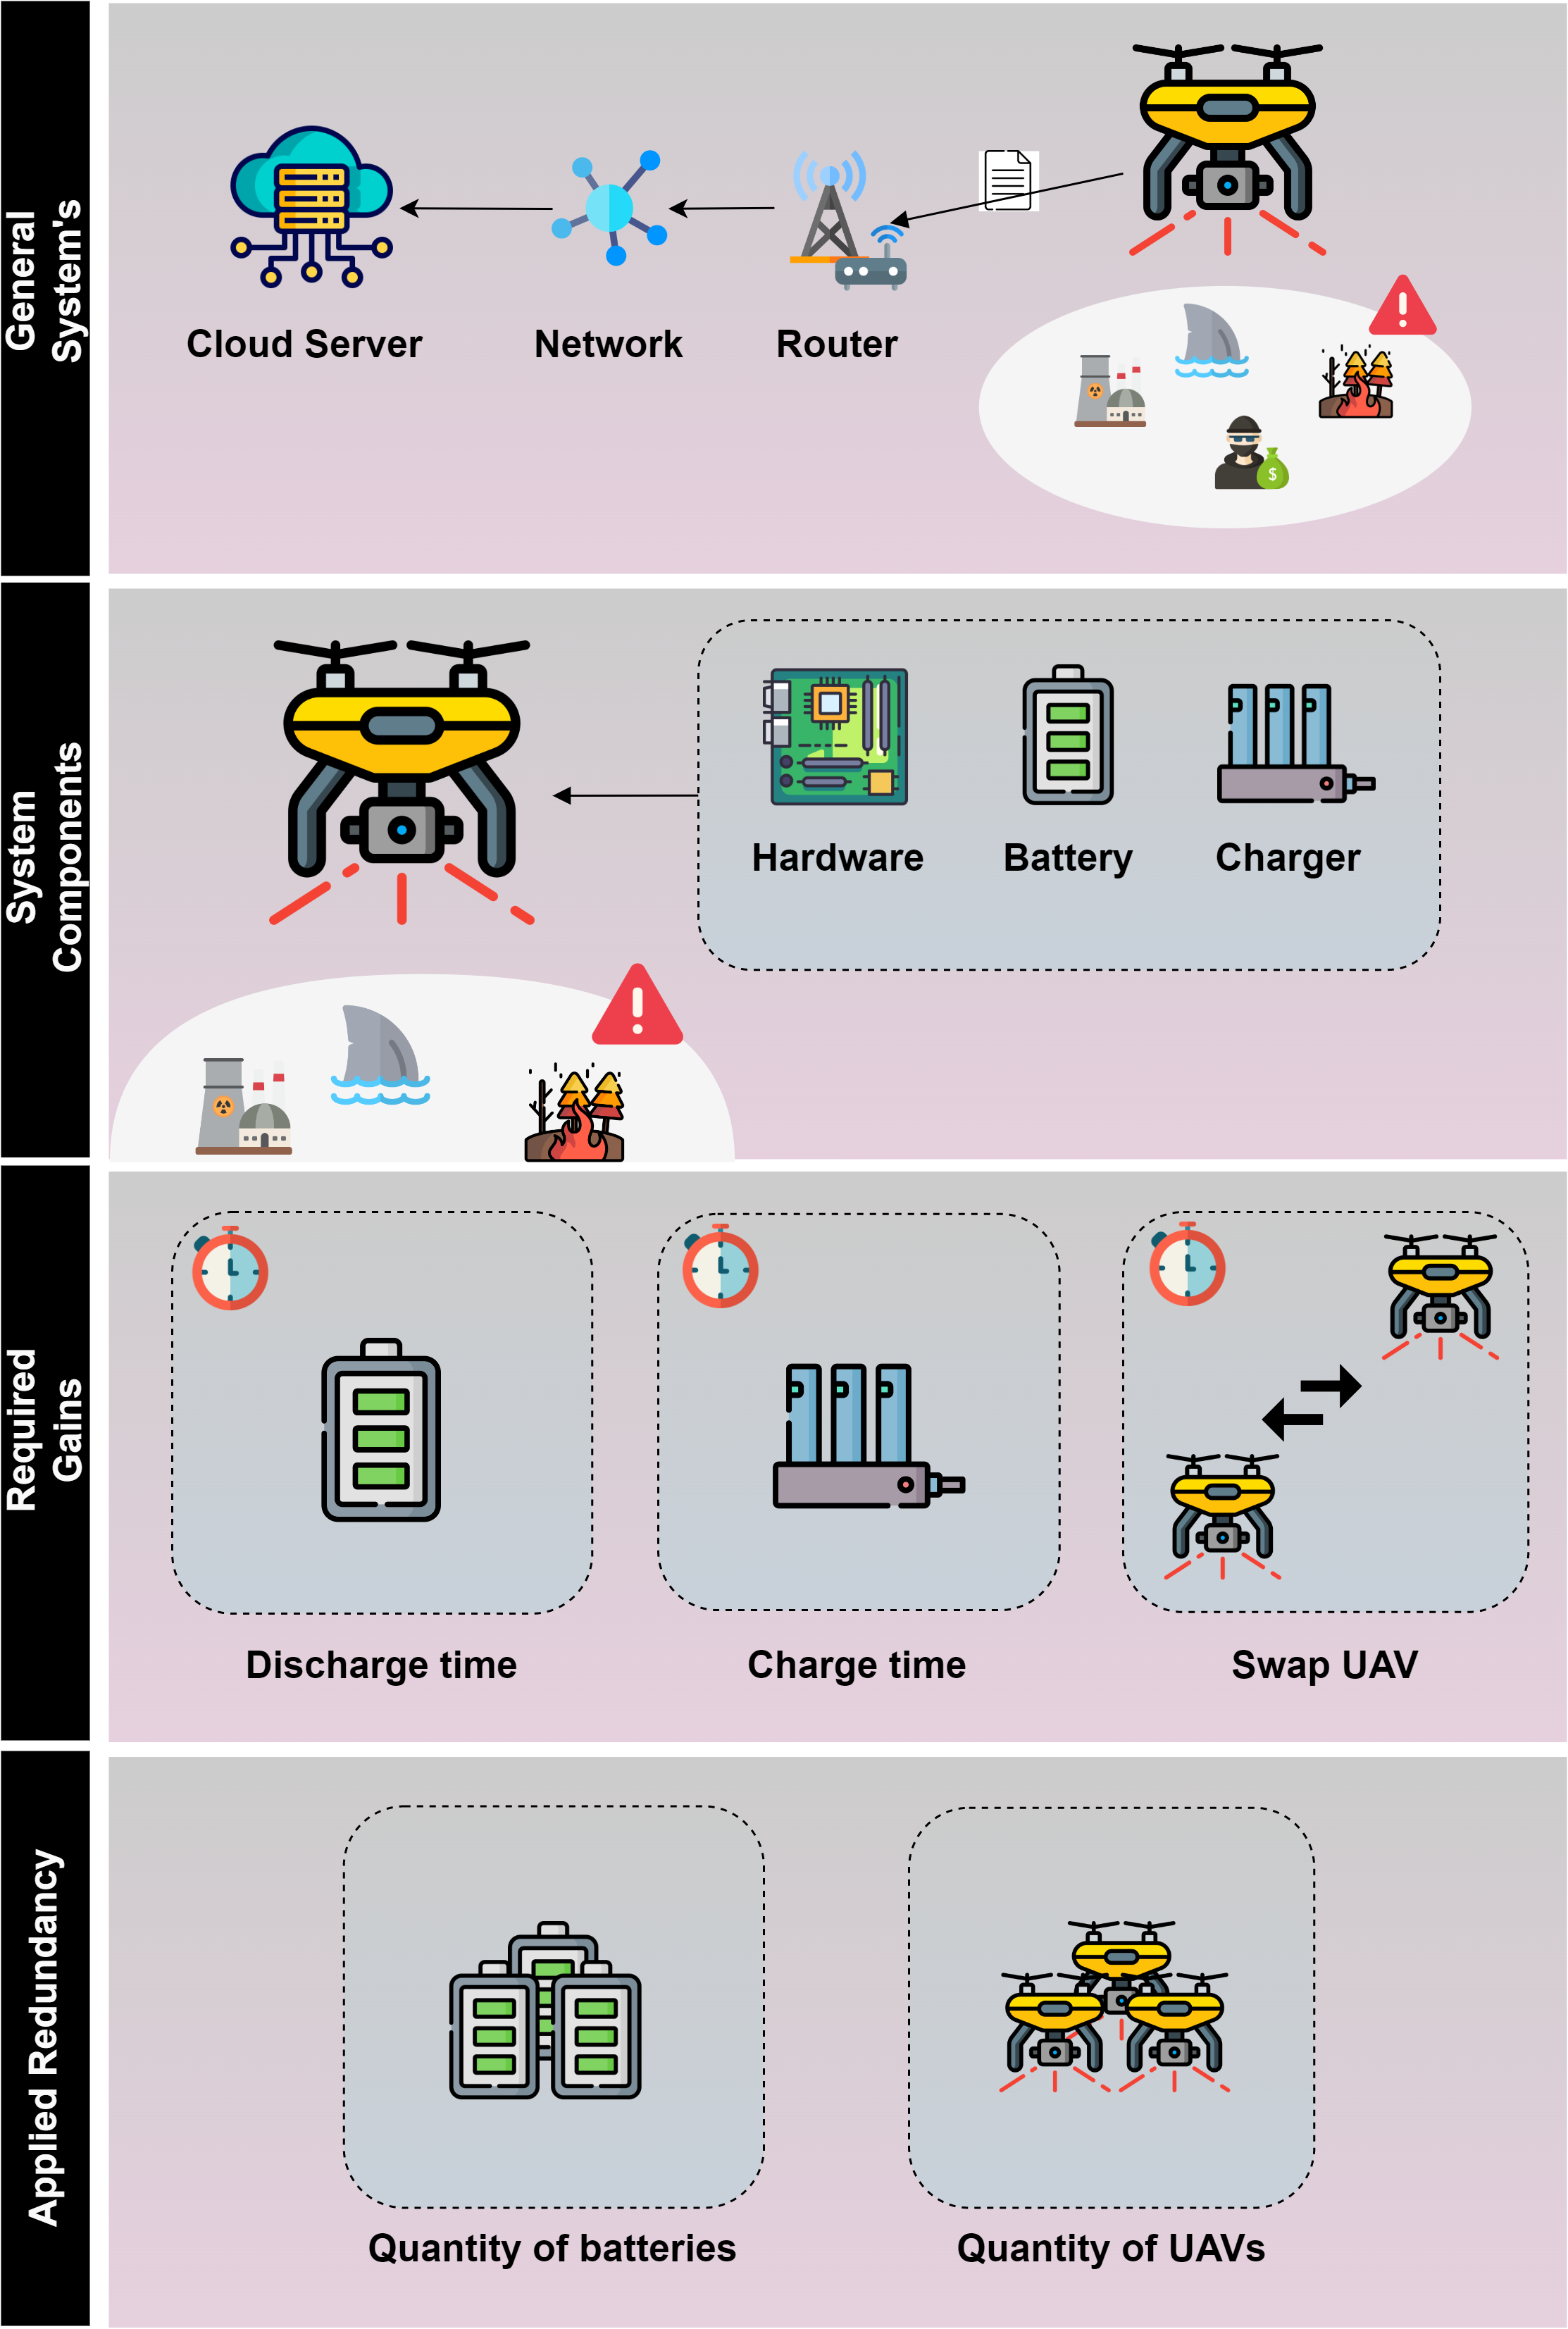
\includegraphics[scale=0.45]{img/operating_model.png}}
\caption{Overview of the Operating Mode}
\label{fig:operating_mode_overview}
\end{figure}

In \textit{General System}, we have the system's basic functioning, a server for data processing, a UAV device for monitoring, and a router for the connection. The system is operational only if the server, router, and UAV are working. For the UAV device, we assume that it is working if it is in flight.

\textit{System components}, shows the components of a UAV device that directly affect its availability, preventing increased flight times. The energy source (battery), charging system, and UAV hardware are among them.

In \textit{Required Gains} and \textit{Applied Redundancy}, we have improvements in component times and UAV replacement (if considering redundancy methods) that can be applied to the base system to increase overall availability. It is important to note that the improvement in transition time is due to the development of an intelligent transition system that can trigger a reserve UAV before the active UAV returns to a landing base.

\subsection{CTMC baseline model}

Figure \ref{fig:ctmc_model} shows our continuous-time Markov chain model representing the flight system of the UAV device, consisting of a drone in operation (flying drone), a backup drone, and a backup power source. The model evaluates the availability of the flight system, having as input parameters the charging rate ($\lambda_{bc}$) and discharging rate($\lambda_{bd}$) of the drone battery per hour, as well as the rate of device hardware failure ($\mu_{d}$) and repair ($\lambda_{d}$) per hour. In addition, the exchange rate between the operating drone and a backup drone per hour is also considered in $\delta$; this exchange rate includes landing time, battery replacement, and takeoff for return (Table \ref{tab:ctmc_parameter_description}).

\begin{figure}[htbp]
\centerline{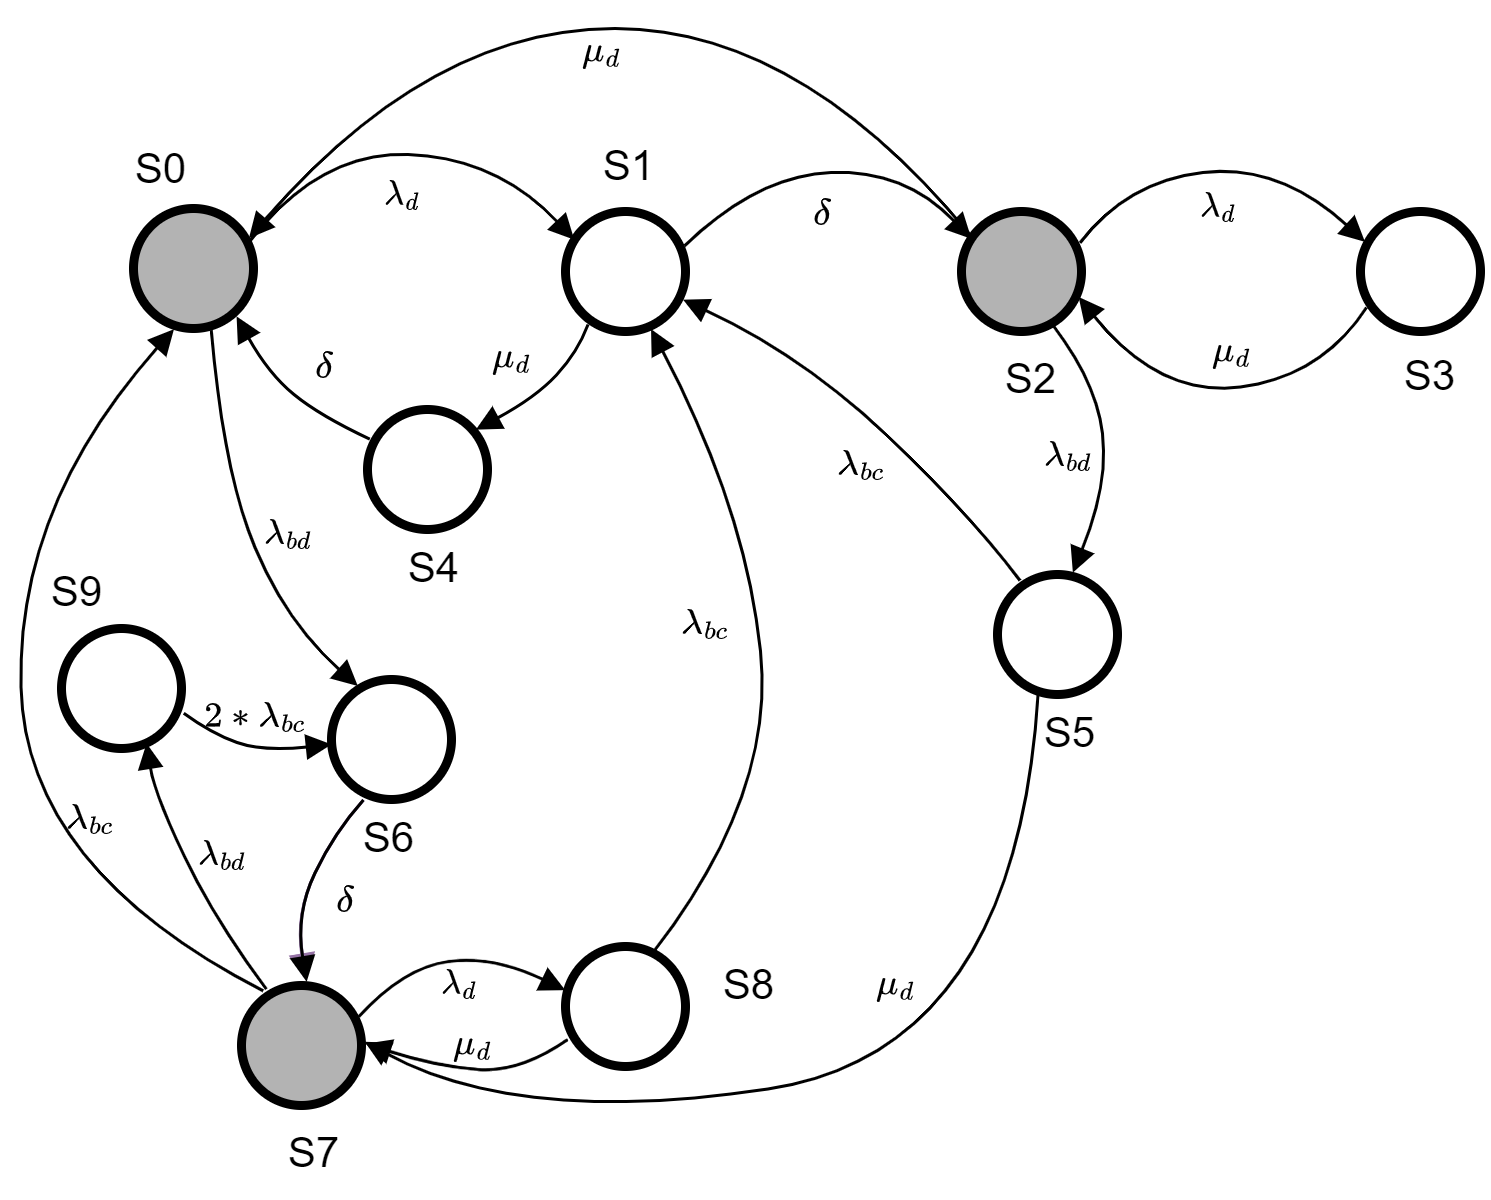
\includegraphics[scale=0.75]{img/CTMC_transparent.png}}
\caption{CTMC model of UAV flight system}
\label{fig:ctmc_model}
\end{figure}

\begin{table}[htbp]
\caption{Parameter Description for the CTMC model}
\begin{center}
\begin{tabular}{c|c}
\hline
\textbf{\textit{Parameter}}& \textbf{\textit{Description}} \\
\hline
\hline
  \(\lambda_{bd}\) & Battery discharge rate per hour \\
  \(\lambda_{bc}\)  & Battery charge rate per hour\\
 \(\mu_{d}\) & Drone repair rate per hour  \\
 \(\lambda_{d}\) & Drone failure rate per hour \\
 \(\delta\) & Drone swap rate per hour \\
\hline
\end{tabular}
\label{tab:ctmc_parameter_description}
\end{center}
\end{table}

In the circle formula, we have the possible states being reached by the system; states illustrated in a dark color as the set of states $\{S0, S2, S7\}$ representing the operating system, that is, when at least one drone is flying over the area of interest or processing the information. Therefore, the other states represent the system offline, with some drones broken or unloaded and no drones or power sources to replace.

From this Markov chain model, we could extract the analytical model, which will serve as a basis for architects and designers in constructing a system with these characteristics. Furthermore, we are considering exponentially distributed times, which makes it possible to extract the closed formula illustrated by the equation \ref{eq:a_uav}.

\begin{align}\label{eq:a_uav}
A_{UAV} = \frac{\delta  \lambda_{bc} \mu_{d} (\alpha_{2} \delta \phi_{2} + \beta_{2} \mu_{d} \phi_{1})}{ \alpha_{2} \delta^{2} \theta_{2} + \lambda_{bc} \mu_{d} (\alpha_{3} \delta  \lambda_{bc} \lambda_{bd} \lambda_{d} + \theta_{1} \mu_{d})+ \beta_{2} \mu_{d}^{3} \phi_{3}}
\end{align}

Where: \\

\begin{minipage}{.8\textwidth}%  
\(\beta = \lambda_{bd} + \lambda_{d};\) \\
\(\beta_{2} = \lambda_{bd} + \mu_{d};\) \\
\(\beta_{3} = \lambda_{d} + \mu_{d};\) \\
\(\beta_{4} = \lambda_{bc} + \lambda_{bd};\) \\
\(\beta_{5} = \lambda_{bc} + \mu_{d};\) \\
\(\alpha_{1} = \beta + \lambda_{bc};\) \\
\(\alpha_{2} = \beta + \beta_{5};\) \\
\(\alpha_{3} = \beta_{3} + \beta_{4};\) \\
\(\alpha_{4} = \beta_{3}\lambda_{bc} + \lambda_{bd} \mu_{d};\) \\
\(\phi_{1} = \alpha_{1}\lambda_{bc} + \beta_{4} \mu_{d};\) \\
\(\phi_{2} = \beta_{3}\lambda_{bc} + \lambda_{bd} \mu_{d};\) \\
\(\phi_{3} = \beta \lambda_{bc}^{2} + \lambda_{bd} (\lambda_{bd} (\delta + \lambda_{bc}) + 2 \delta \lambda_{bc});\) \\
\(\phi_{4} = \beta_{3}^{2} + \beta_{3} (\lambda_{bc} + 3 \lambda_{bd}) + \lambda_{bd} (2 \lambda_{bc} + 3 \lambda_{bd});\) \\
\(\phi_{5} = \lambda_{d}^{2} + \lambda_{d} \mu_{d} + \mu_{d}^{2} ;\) \\
\(\theta_{1} = \alpha_{1} \beta  \beta_{2} \lambda_{bc} + 2 \beta  \beta_{2}  \delta \lambda_{bd}+ \delta  \lambda_{bc} \phi_{4};\) \\
\(\theta_{2} =  \alpha_{4} \lambda_{bd} \mu_{d} + \lambda_{bc}^{2} \phi_{5};\) \\
\end{minipage}%

We also include the formula for the availability of other components necessary for the functioning of a monitoring system like this, composed of a server and a connection device exemplified here as a router, its analytical formulas being shown in the equations \ref{eq:a_server} and \ref{eq:a_router}, respectively. However, we do not consider them in our sensitivity analyses and in assessing system availability. This is because components such as the server and the router have high availability compared to the UAV device, considered by us as the major bottleneck of the overall system and selected for availability improvement analysis.

\begin{align}
\label{eq:a_server}
A_{Server} = \frac{\lambda_{hw}}{\lambda_{hw} + \mu_{hw}} \times \frac{\lambda_{os}}{\lambda_{os} + \mu_{os}} \times
\frac{\lambda_{hp}}{\lambda_{hp} + \mu_{hp}} 
\end{align}

\[\times(1- (\frac{\mu_{vm}}{\lambda_{vm} + \mu_{vm}})^{3})\]

\begin{align}
\label{eq:a_router}
A_{R} = \frac{\lambda}{\lambda + \mu} 
\end{align}

The analytical model of server availability (Equation \ref{eq:a_server}) and router (Equation \ref{eq:a_router}) has in its structure the failure rate, represented by $\lambda$ and the repair rate $\mu $. However, the server availability model is composed of the product of the hardware availability models ($hw$), operating system ($os$), virtual machine management hypervisor ($hp$), and virtual machine model ($vm$); components commonly used for processing a monitoring system.

\begin{align}\label{eq:a}
A = A_{Server} \times A_{R}  \times A_{UAV}
\end{align}

The system's general availability is given by Equation \ref{eq:a}, where we have the product of the server, router, and UAV flight system availability models.

\subsection{SPN redundancy model}

The UAV flight system availability analytical model (Equation \ref{eq:a_uav}) extracted from CTMC considers only the system in basic operating mode, i.e., one in-flight UAV, one backup UAV, and one backup battery. As already seen, we can use it to vary the failure and repair times of the UAV, battery, and recharging components to improve the availability metric. However, to include redundancy mechanisms in this model and have a system with a more advanced operating mode, we would have a model with a huge state space for calculating availability.

Given the problem of giant state space in Markov chains and analytical models extracted from it impossible to be calculated by a person, we then propose an approach with a numerical method model of stochastic Petri nets (SPN) that can be evaluated using computational tools such as Mercury \cite{maciel2017mercury}.

The SPN model represented by Figure \ref{fig:spn_model} was used to model the use of redundancy mechanisms in the system. The place (circle) \textbf{DU} marks the system as working, while the place \textbf{DF} indicates a failed state. The other places: \textbf{DR}, \textbf{BR}, and \textbf{BC}, indicate the number of spare UAVs, spare batteries, and charging batteries, respectively.

\begin{figure}[htbp]
\centerline{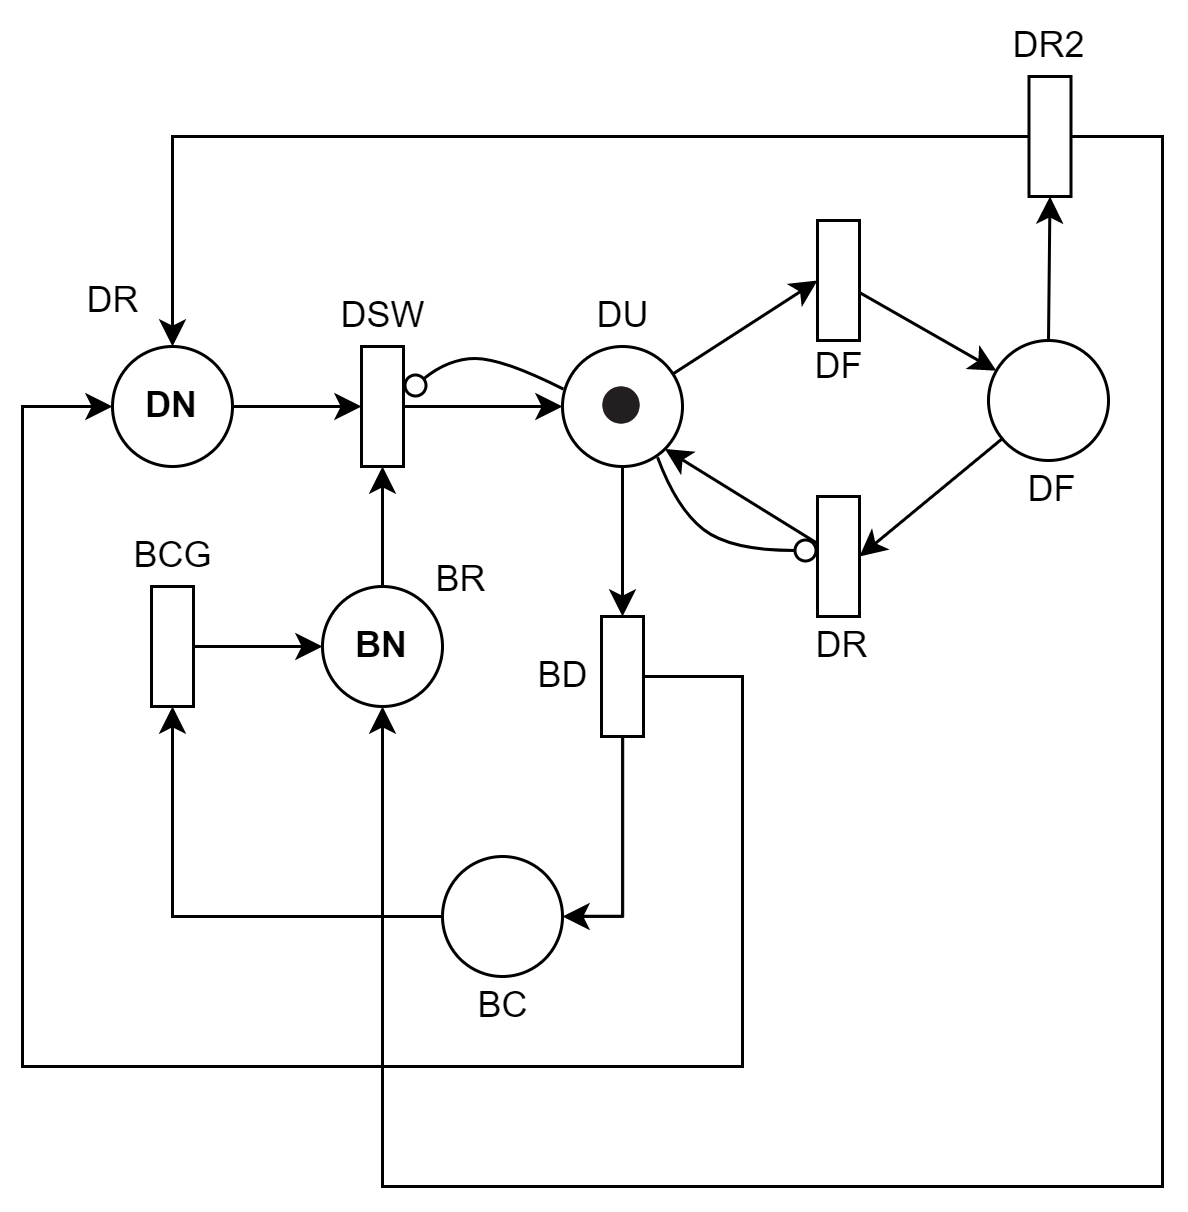
\includegraphics[scale=0.7]{img/SPN_transparent.png}}
\caption{SPN model of UAV flight system}
\label{fig:spn_model}
\end{figure}

Initially, 1 UAV is operational, with one backup UAV and one backup battery. The UAV has a mean time to failure (MTTF) and a mean time to repair (MTTR), as well as an average recharge, discharge, and swapping time. These times follow an exponential distribution, represented in the model by timed transitions (white rectangles) connected by arcs to the state places. All meantime parameters (MTTs) used as input to the model can be seen in Table \ref{tab:spn_parameter_description} per associated transition.

\begin{table}[htbp]
\caption{Parameter Description for the SPN model}
\begin{center}
\begin{tabular}{c|c|c}
\hline
\textbf{\textit{Transition}} & \textbf{\textit{Parameter}}& \textbf{\textit{Description}} \\
\hline
\hline
 DF & MTTFD & Mean time to drone failure \\
 DR & MTTRD & Mean time to drone repair\\
 DR2 & MTTRD & With guard \textbf{$\#DU>0$} \\
 BD & MTTBD & Mean time to battery discharge \\ 
 BCG & MTTBC & Mean time to battery charge \\
 DSW & MTTDS & Mean time to drone swap  \\
\hline
\end{tabular}
\label{tab:spn_parameter_description}
\end{center}
\end{table}

There are two types of arcs in the proposed model; the arc that ends with an arrow is the most common and indicates the activation of a transition if the requirements are met and the movement of a token (the small black circle inside a place, which shows the number of features). The arc that ends with a circle is called an inhibitory arc. An inhibitor arc indicates that a transition can only be activated if the origin place of the arc is empty; in the specific model, it allows only one active UAV at a time and determines if a spare or recovered UAV can assume the position if it satisfies the condition. On the other hand, timed transitions depend on the time to activate. Finally, those with a black rectangle, called immediate transition, can be triggered if the required tokens are present at the connected location \citep{melo2021distributed}.

%-----------------------------------------------------------------------------------------------
\section{Results and Case Studies}
\label{sec:case_studies}

This section presents a sensitivity analysis of the UAV flight system components through the percentage differentiation technique defined by Equation \ref{eq:sa}. Next, we show a sensitivity ranking, where the precedence of the parameters reflects the significance of their impact on the system availability metric (Table \ref{tab:sa_rank}). These values guide us on which components need improvement and define our case studies.

\begin{table}[htbp]
\caption{Sensitivity ranking}
\begin{center}
\begin{tabular}{c|c|c}
\hline
\textbf{\textit{Parameter}}& \textbf{\textit{Ranking}} & \textbf{\textit{Sensitivity index}} \\
\hline
\hline
\(\lambda_{bd}\) & \(1^{st}\) & -3.720460029055 \\
\(\lambda_{bc}\) & \(2^{nd}\) & 3.3226751100809997 \\
 \(\mu_{d}\) & \(3^{rd}\) & -1.064622392094 \\
\(\lambda_{d}\) & \(4^{th}\) & 0.9995887722079999 \\
\(\delta\) & \(5^{th}\) & 0.462793032533 \\
\hline
\end{tabular}
\label{tab:sa_rank}
\end{center}
\end{table}

In \textit{Case Study \#1}, we analyzed the impact of varying times (MTTs) of battery discharge, charging, and drone switching on the system availability metric, having the baseline system as the initial configuration. 
%
\textit{Case Study \#2} analyzes the impact of increasing redundant components considering the redundancy technique applied with the system availability metric, having the baseline system as the initial configuration. 
%
\textit{Case Study \#3} uses the time improvement applied in case study 1 and evaluates the impact of increasing backup component redundancy given initial improvements. This combination of the two methods used in Case Studies 1 and 2 can be considered to decrease costs, having a compromise between improvements and the addition of redundant components.

%\subsection{Sensitivity analysis}

In our ranking, built through the sensitivity analysis performed, we have the battery discharge rate per hour as the parameter that most impacts the system availability according to the sensitivity index of column 3 of Table \ref{tab:sa_rank}, followed by the charging rate per hour, repair rate, failure rate, and UAV exchange rate.


\subsection{Case Study \#1}
\label{sec:case_studies_sub01}

\begin{figure}[htbp]
\centerline{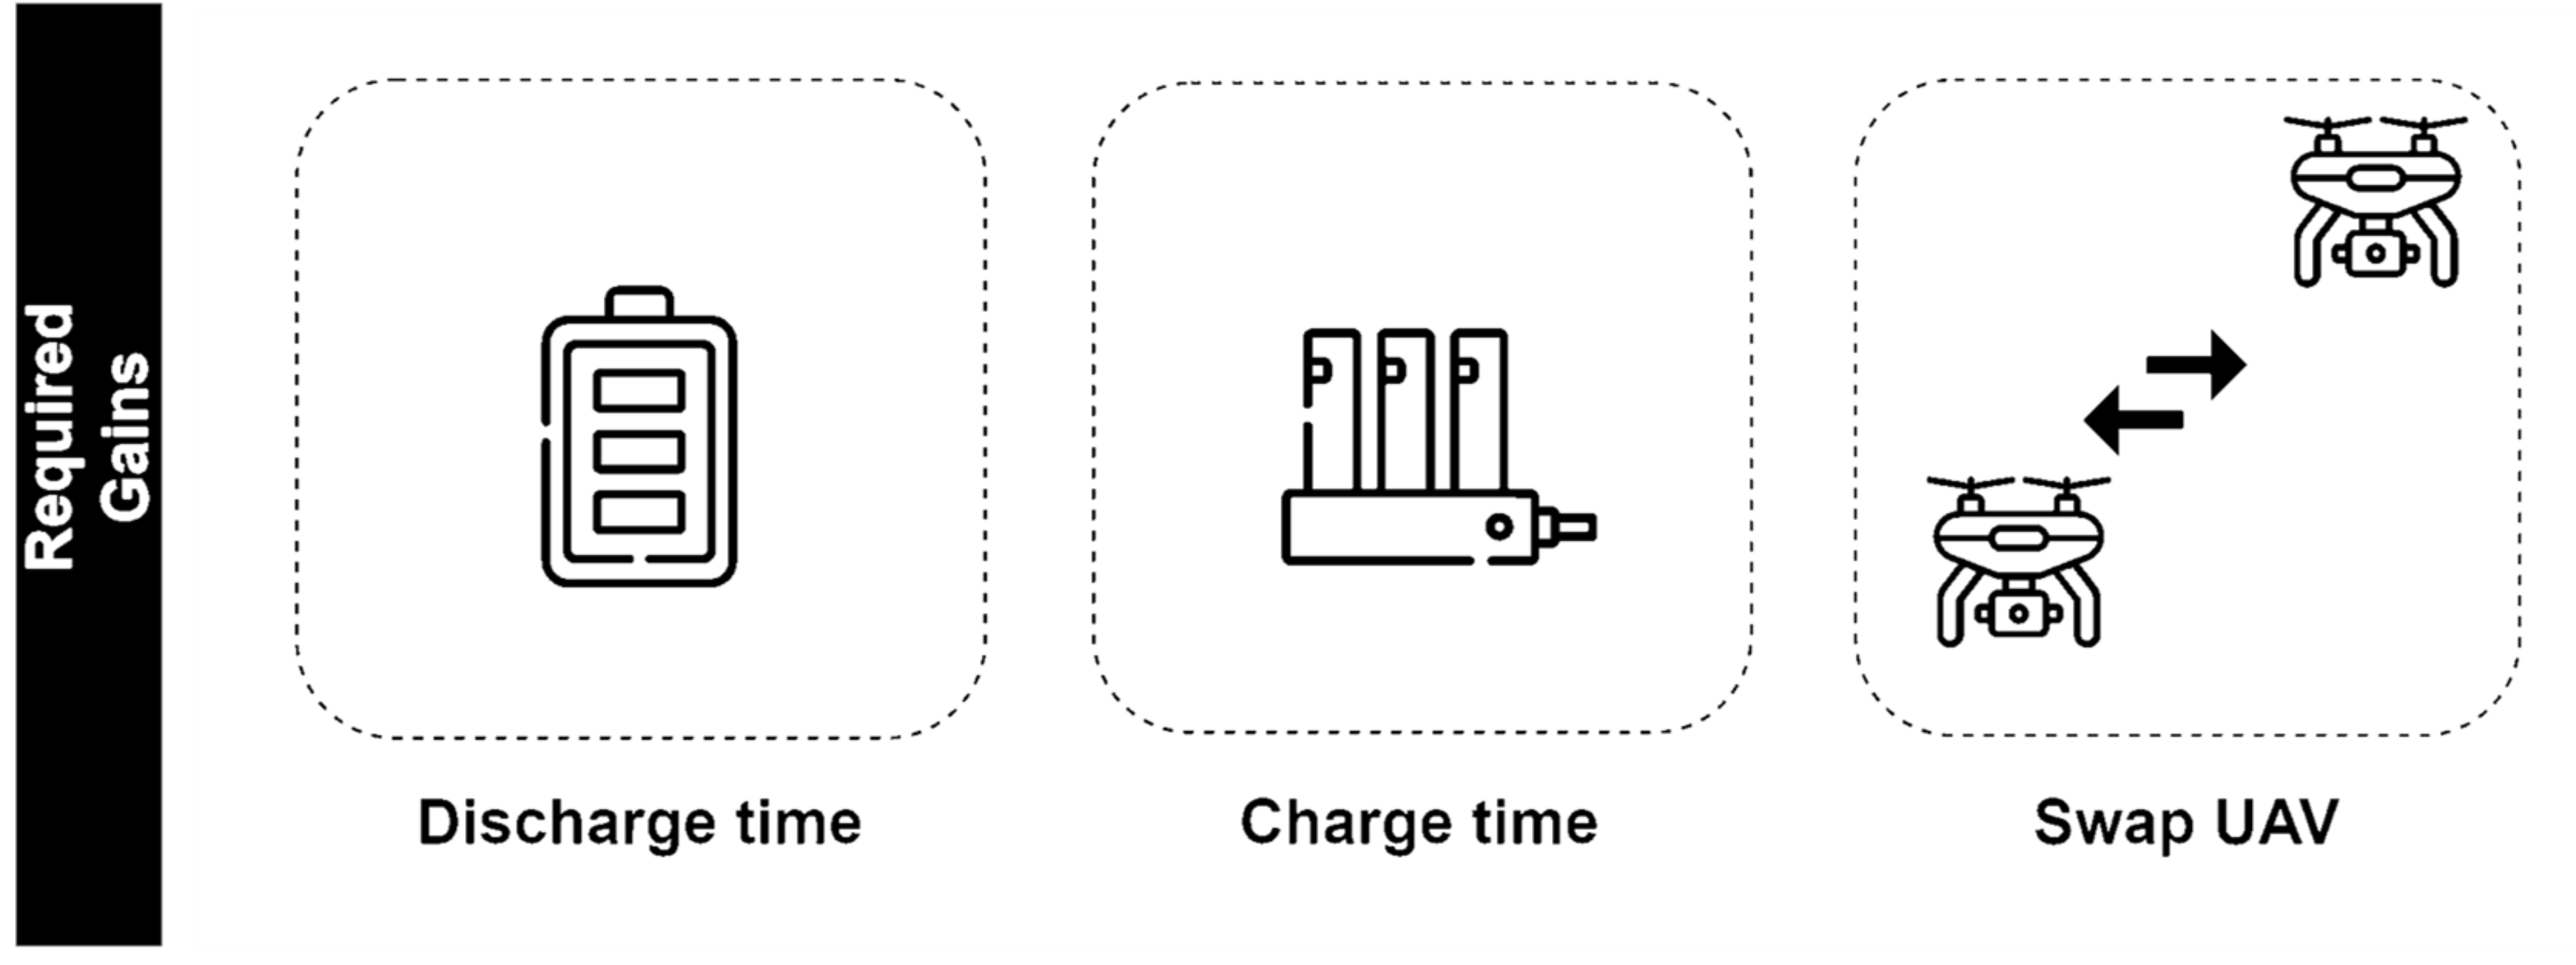
\includegraphics[scale=0.2]{img/operating_model_study_01.png}}
\caption{Required Gains}
\label{fig:case_study_01}
\end{figure}

In this case study, we use the analytical model to assess the possible impacts on availability given improvements in the times of some components used as parameters in the model (Fig.\ref{fig:case_study_01}). System baseline parameter values are shown in Table \ref{tab:ctmc_parameter_values}.

\begin{table}[htbp]
\caption{Parameter values for the CTMC model}
\begin{center}
\begin{tabular}{c|c}
\hline
\textbf{\textit{Parameter}} & \textbf{\textit{Value (rate)}} \\
\hline
\hline
  $\lambda_{bd}$  & 2 \\
  $\lambda_{bc}$   & 0.5 \\
  $\mu_{d}$   & 0.5  \\
  $\lambda_{d}$ & 0.0002 \\
  $\delta$  & 6 \\
\hline
\end{tabular}
\label{tab:ctmc_parameter_values}
\end{center}
\end{table}


Parameter values are given in rate format (amount per hour) as input to the analytical and illustrated model in the continuous-time Markov chain. Where, $\lambda_{bd}$ means 2 battery discharges per hour, $\lambda_{bc}$ is 0.5 charges per hour, $\mu_{d}$ 0.5 repairs per hour, $\lambda_{d}$ is 0.0002 failures per hour and $\delta$ is 6 UAV changes per hour.

We started our analysis by varying the value of $\lambda_{bd}$, fixed this value to the value that resulted in better system availability, and varied the next one, $\lambda_{bc}$. Finally, we vary the swap parameter ($\delta$) with the values of $\lambda_{bd}$ and $\lambda_{bc}$ fixed their enhanced values.

The values $\lambda_{d}$ and $\mu_{d}$, repair rate, and failure rate of the UAV were not evaluated in this study. Their values were ignored because we considered the improvement and maintenance of UAV equipment costly and with little impact on system availability.

Figure \ref{fig:ctmc_sa} presents the time improvements graphs. Figure \ref{fig:ctmc_sa_bd} shows the graph with MTT time improvements of $\lambda_{bd}$. For example, the baseline system of the UAV flight has an availability of 0.34\% with $\lambda_{bd}$ equal to 30 minutes of flight or unloading time; when we improve this time, we have an availability of 0.84\% with a flight time of 180 minutes. In Figure \ref{fig:ctmc_sa_bc}, we have the battery charging time improvement graph, with an availability improvement of 0.90\% for 30 minutes of charging, considering a discharge time of 180 minutes. Finally, we achieved availability of 0.97\% with a UAV changeover of fewer than 1.30 minutes, considering unload and load times fixed at 180 and 30 minutes each (Figure \ref{fig:ctmc_sa_suav}).


\begin{figure}[htbp]
     \centering
     \begin{subfigure}[b]{0.45\textwidth}
         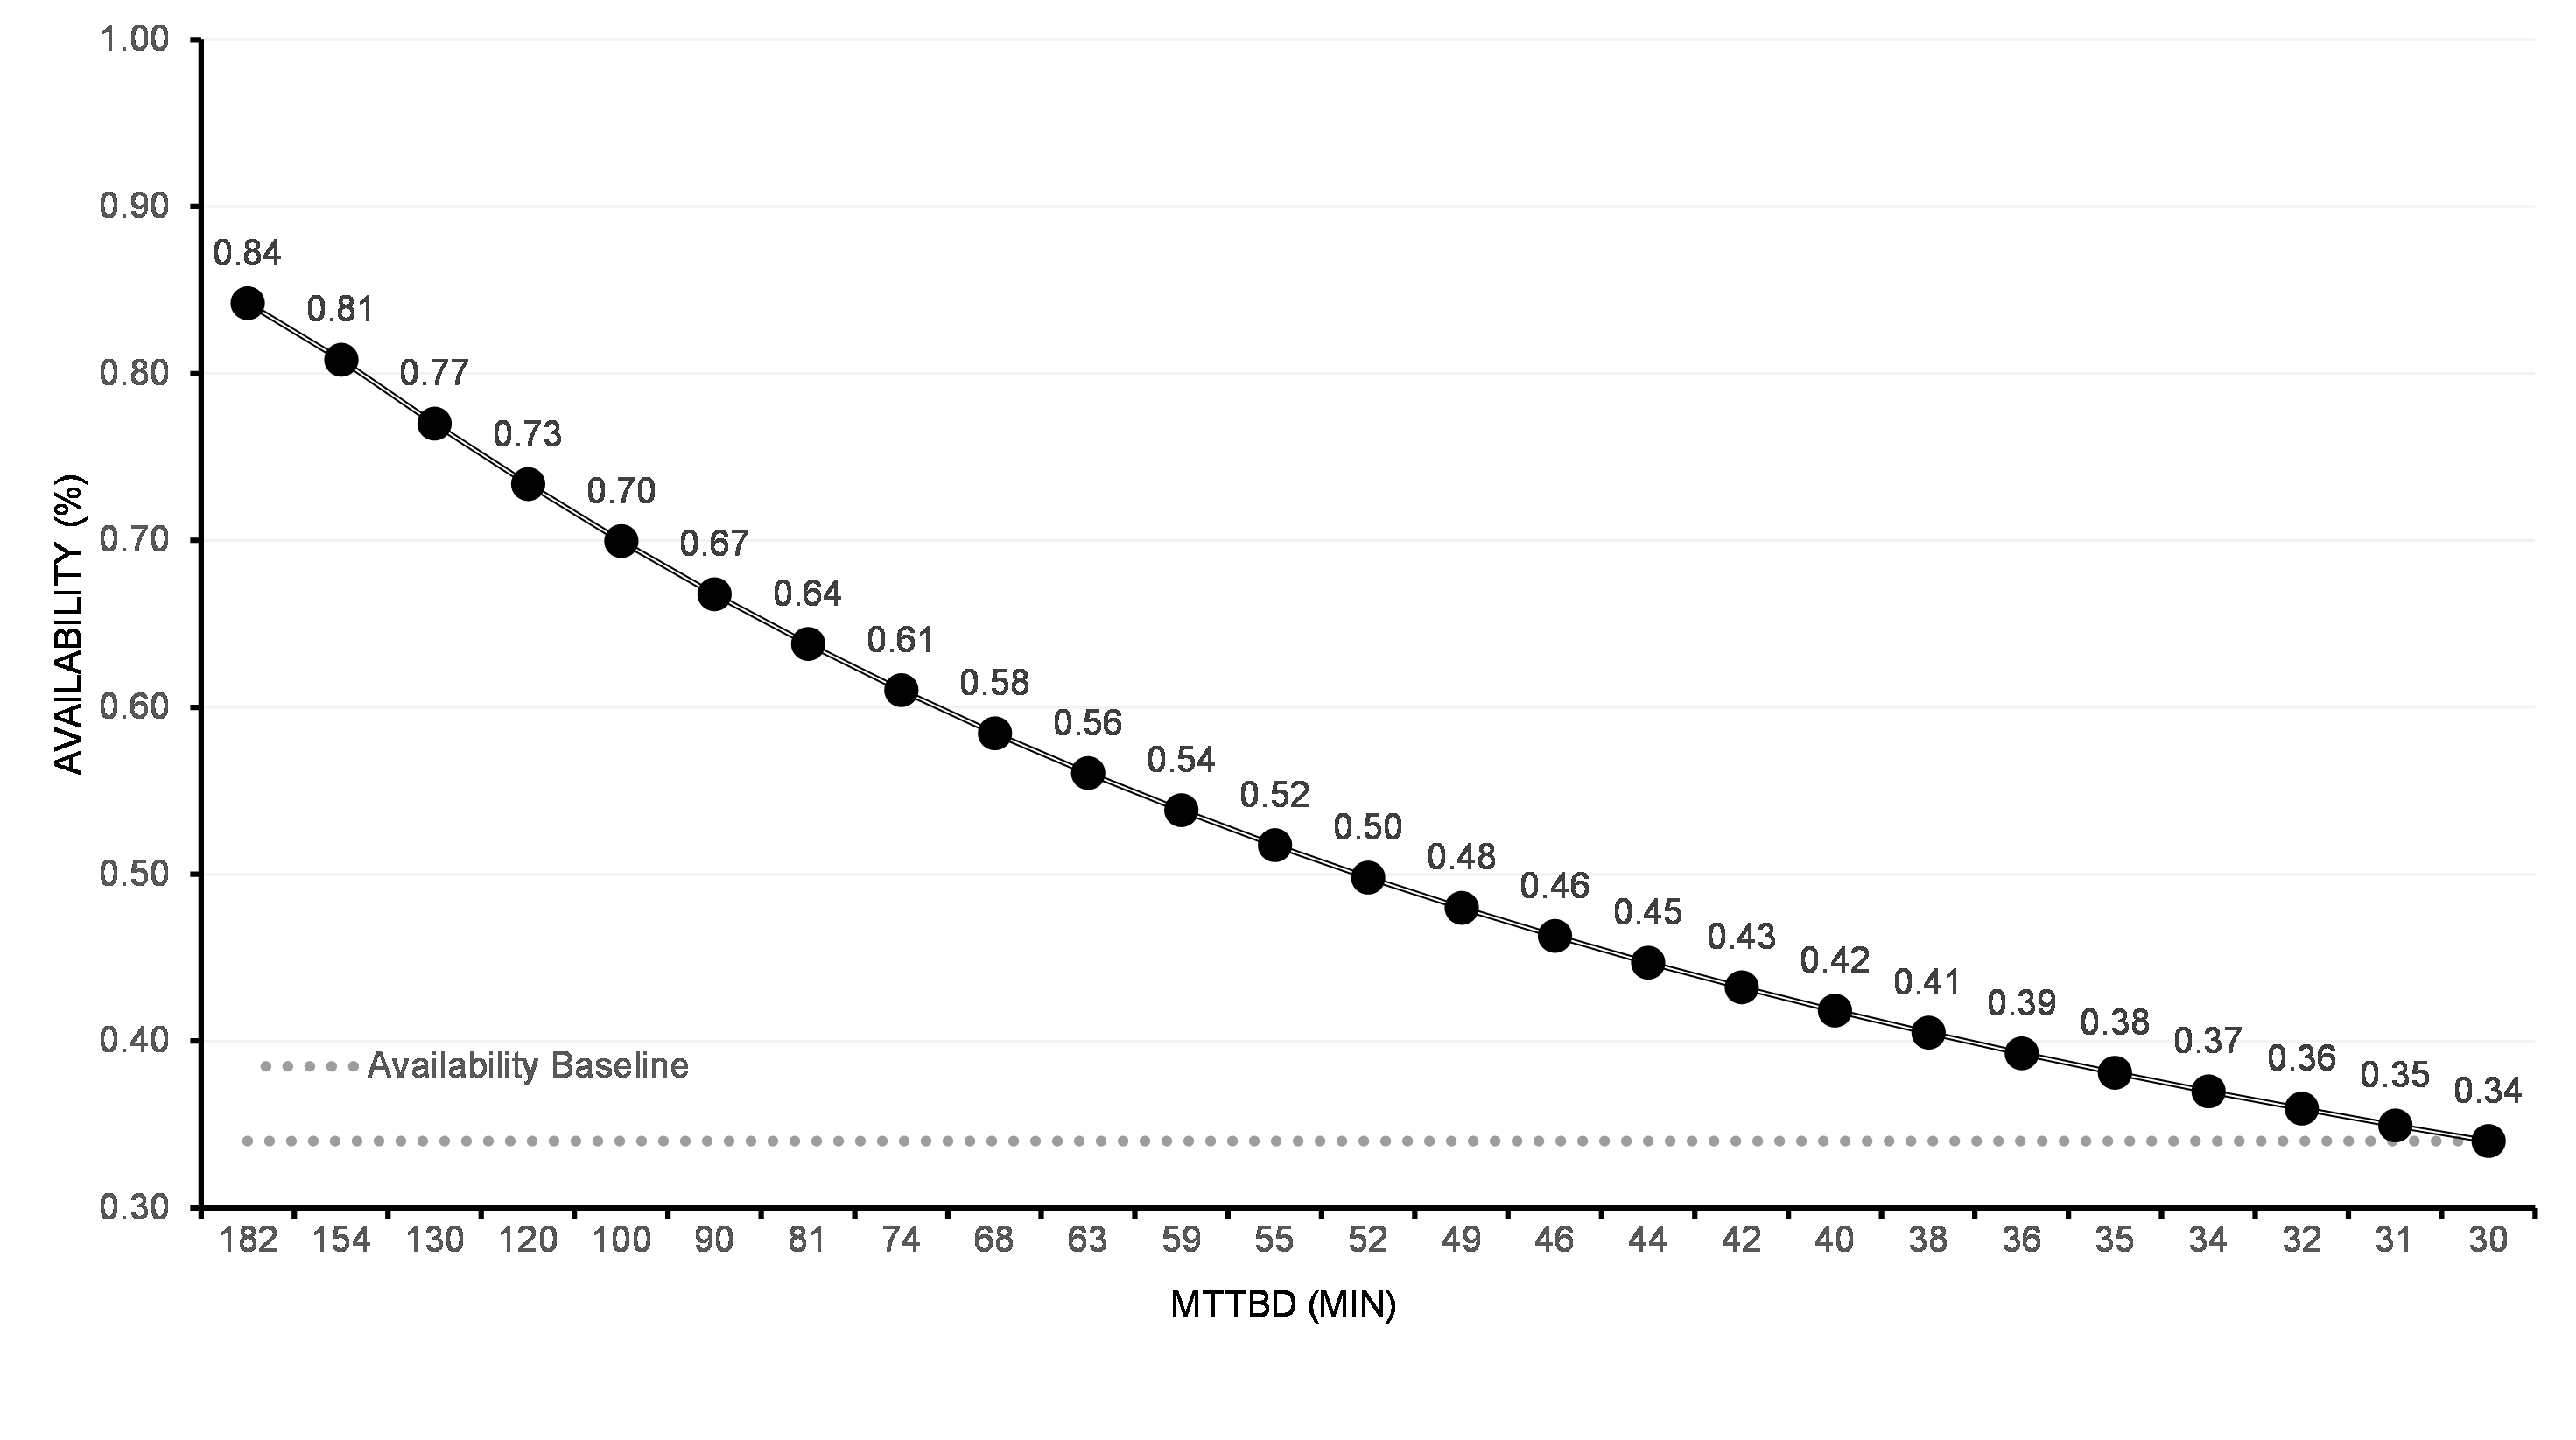
\includegraphics[width=\linewidth]{img/exps/SA_007.png}
         \caption{Mean Time to Battery Discharge}
         \label{fig:ctmc_sa_bd}
     \end{subfigure}
     \hfill
     \begin{subfigure}[b]{0.45\textwidth}
         \centering
         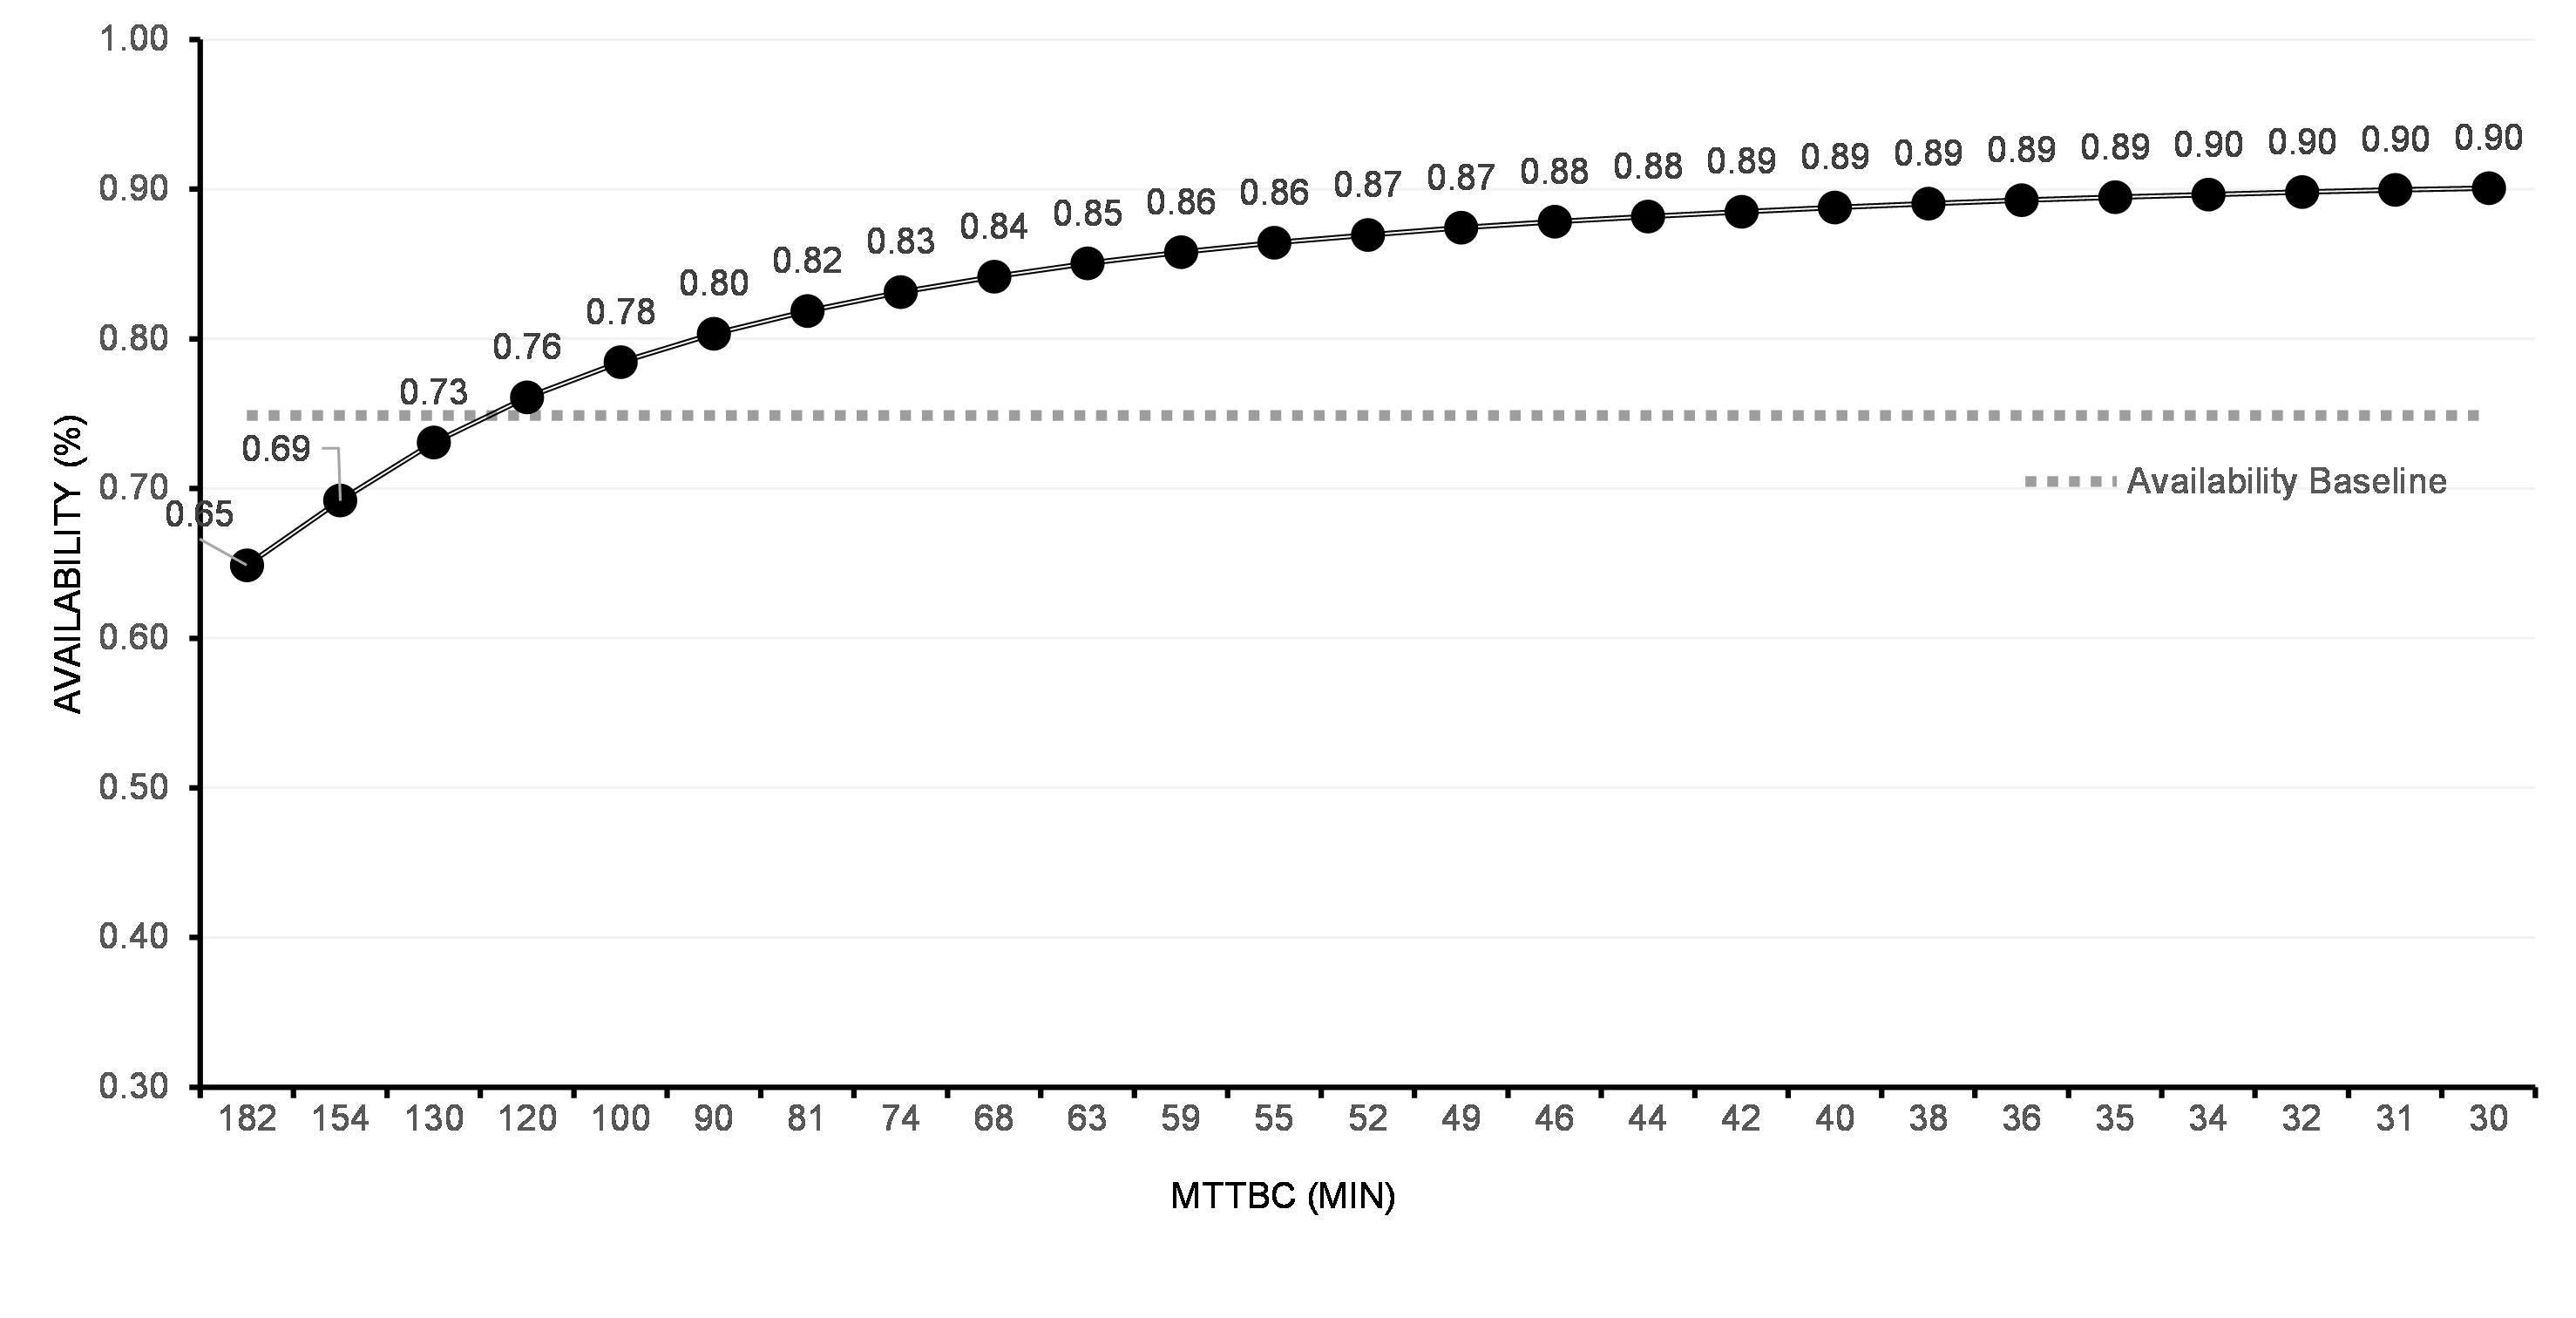
\includegraphics[width=\linewidth]{img/exps/SA_001.png}
         \caption{Mean Time to Battery Charge}
         \label{fig:ctmc_sa_bc}
     \end{subfigure}
     \hfill
     \begin{subfigure}[b]{0.45\textwidth}
         \centering
         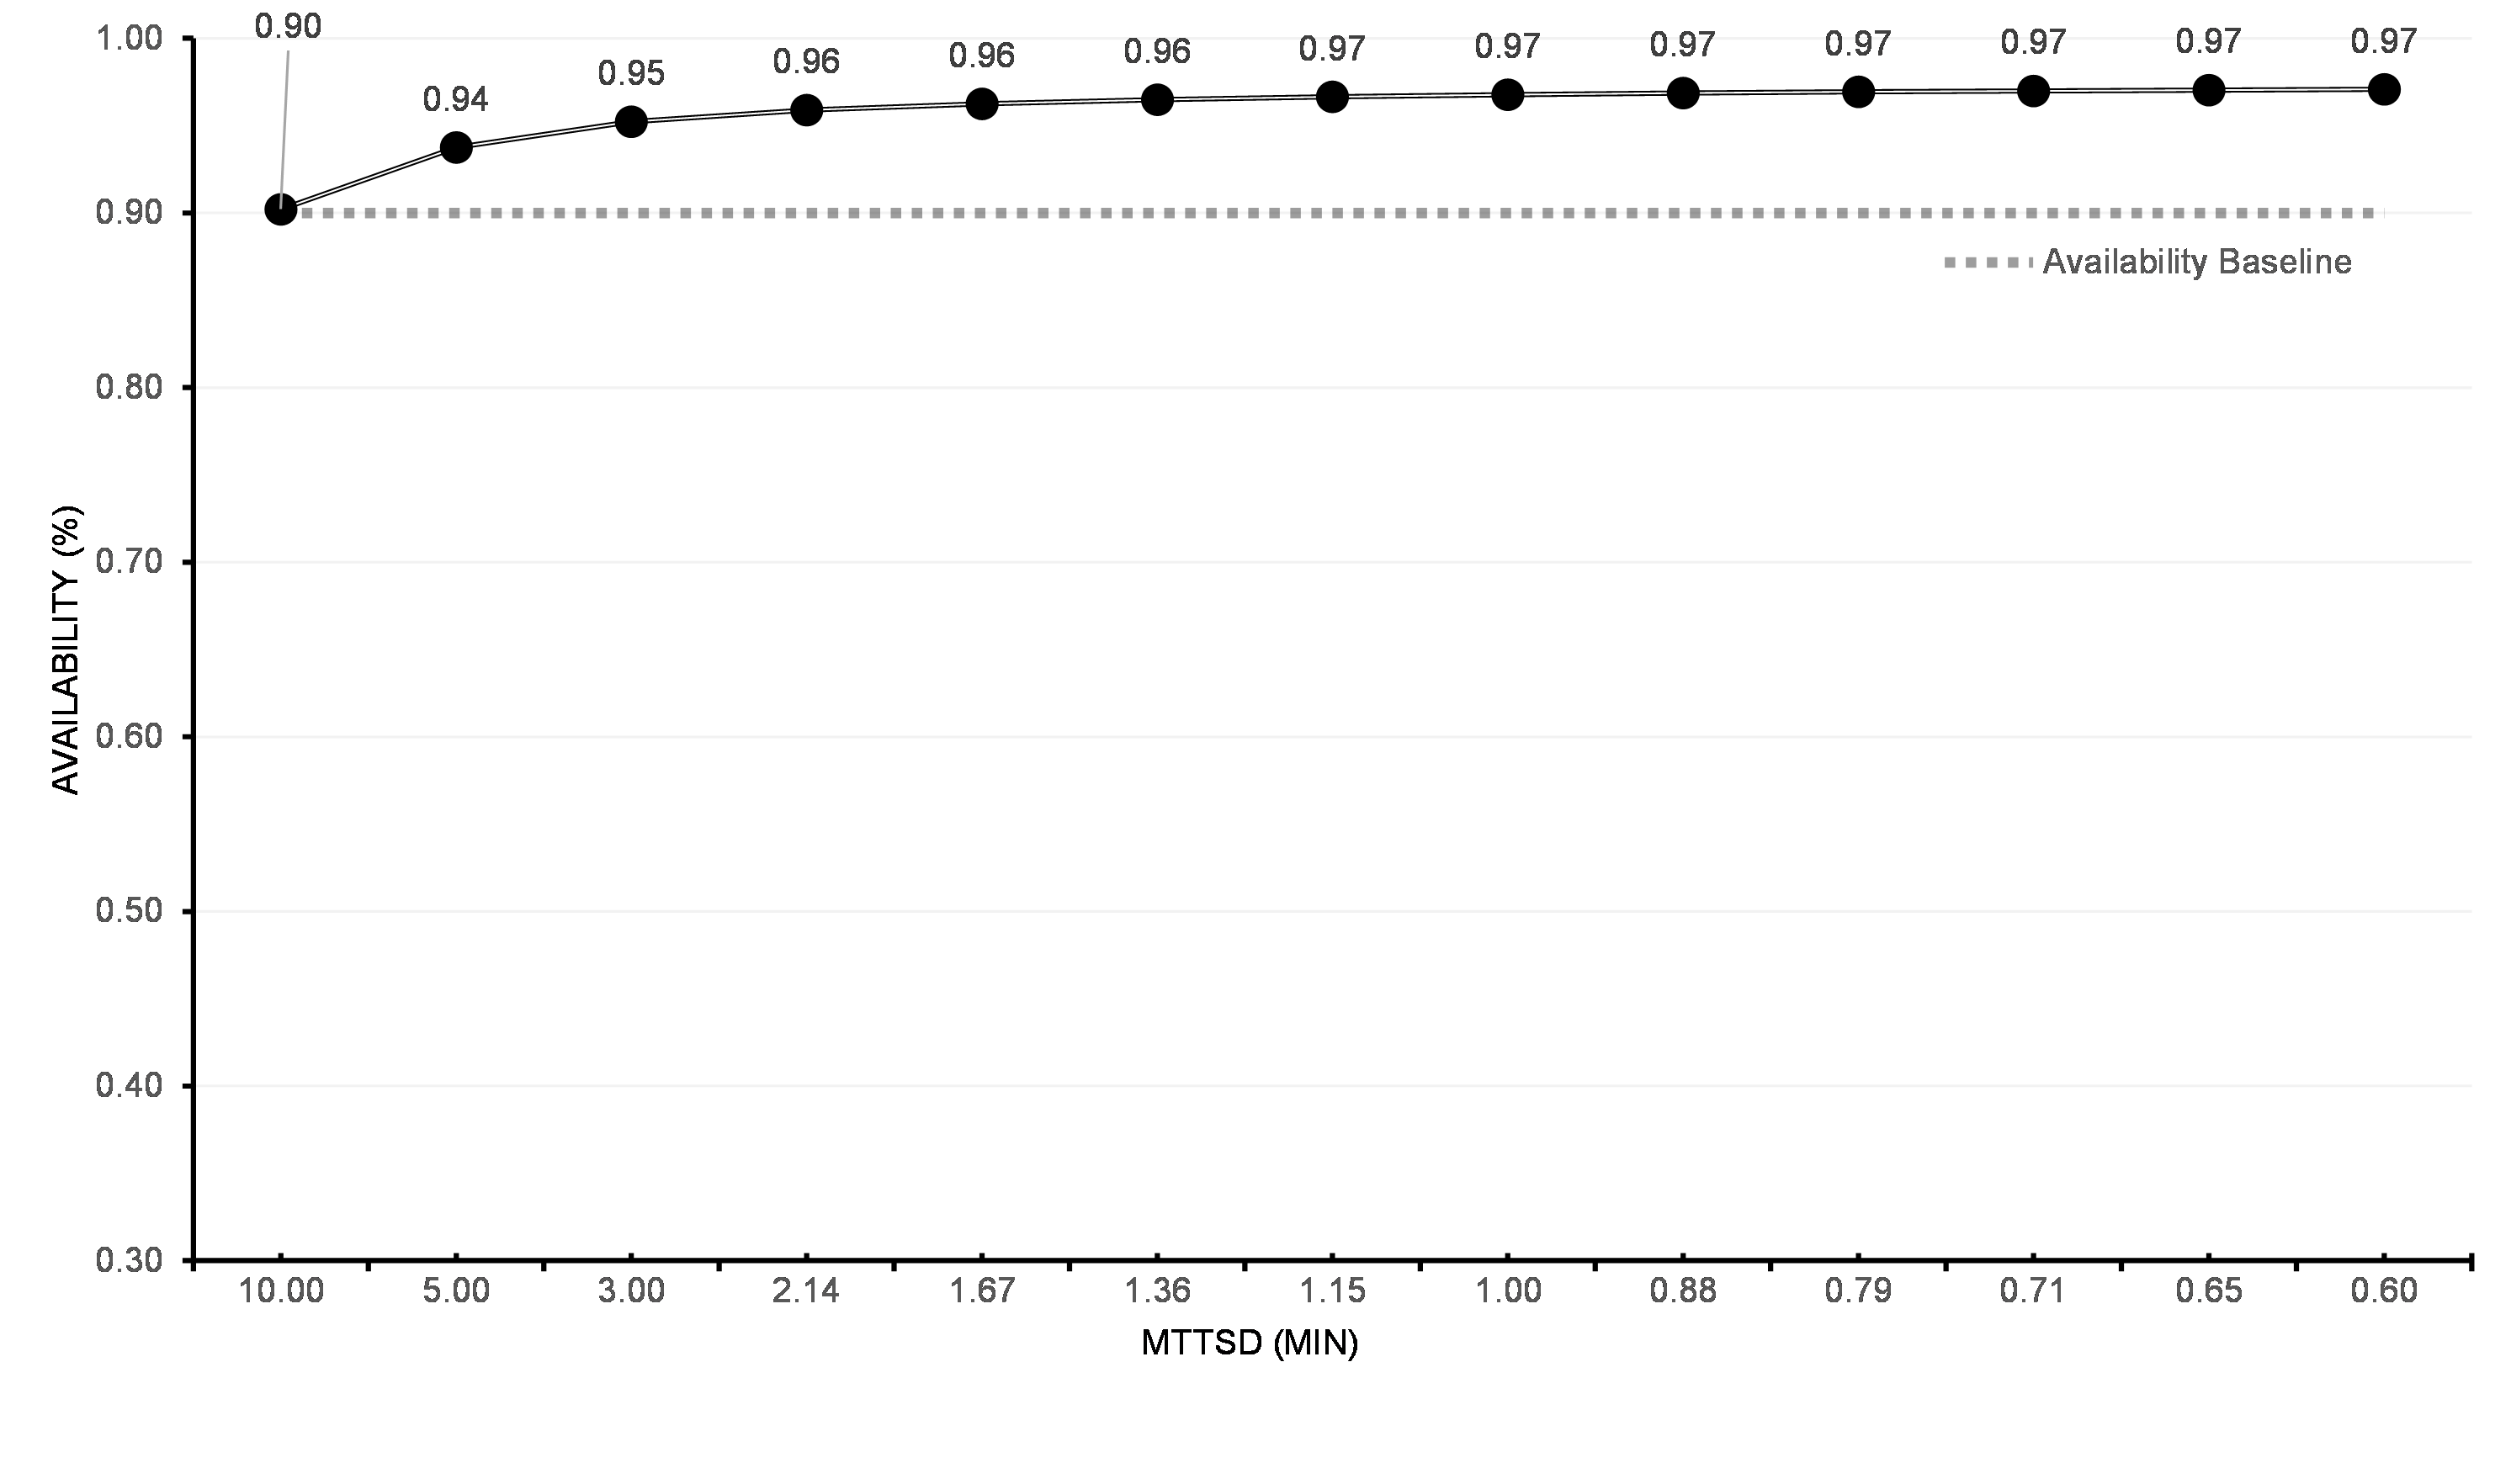
\includegraphics[width=\linewidth]{img/exps/SA_002.png}
         \caption{Mean Time to Drone Swap}
         \label{fig:ctmc_sa_suav}
     \end{subfigure}
        \caption{Time improvements}
        \label{fig:ctmc_sa}
\end{figure}


\subsection{Case Study \#2}
\label{sec:case_studies_sub02}

\begin{figure}[htbp]
\centerline{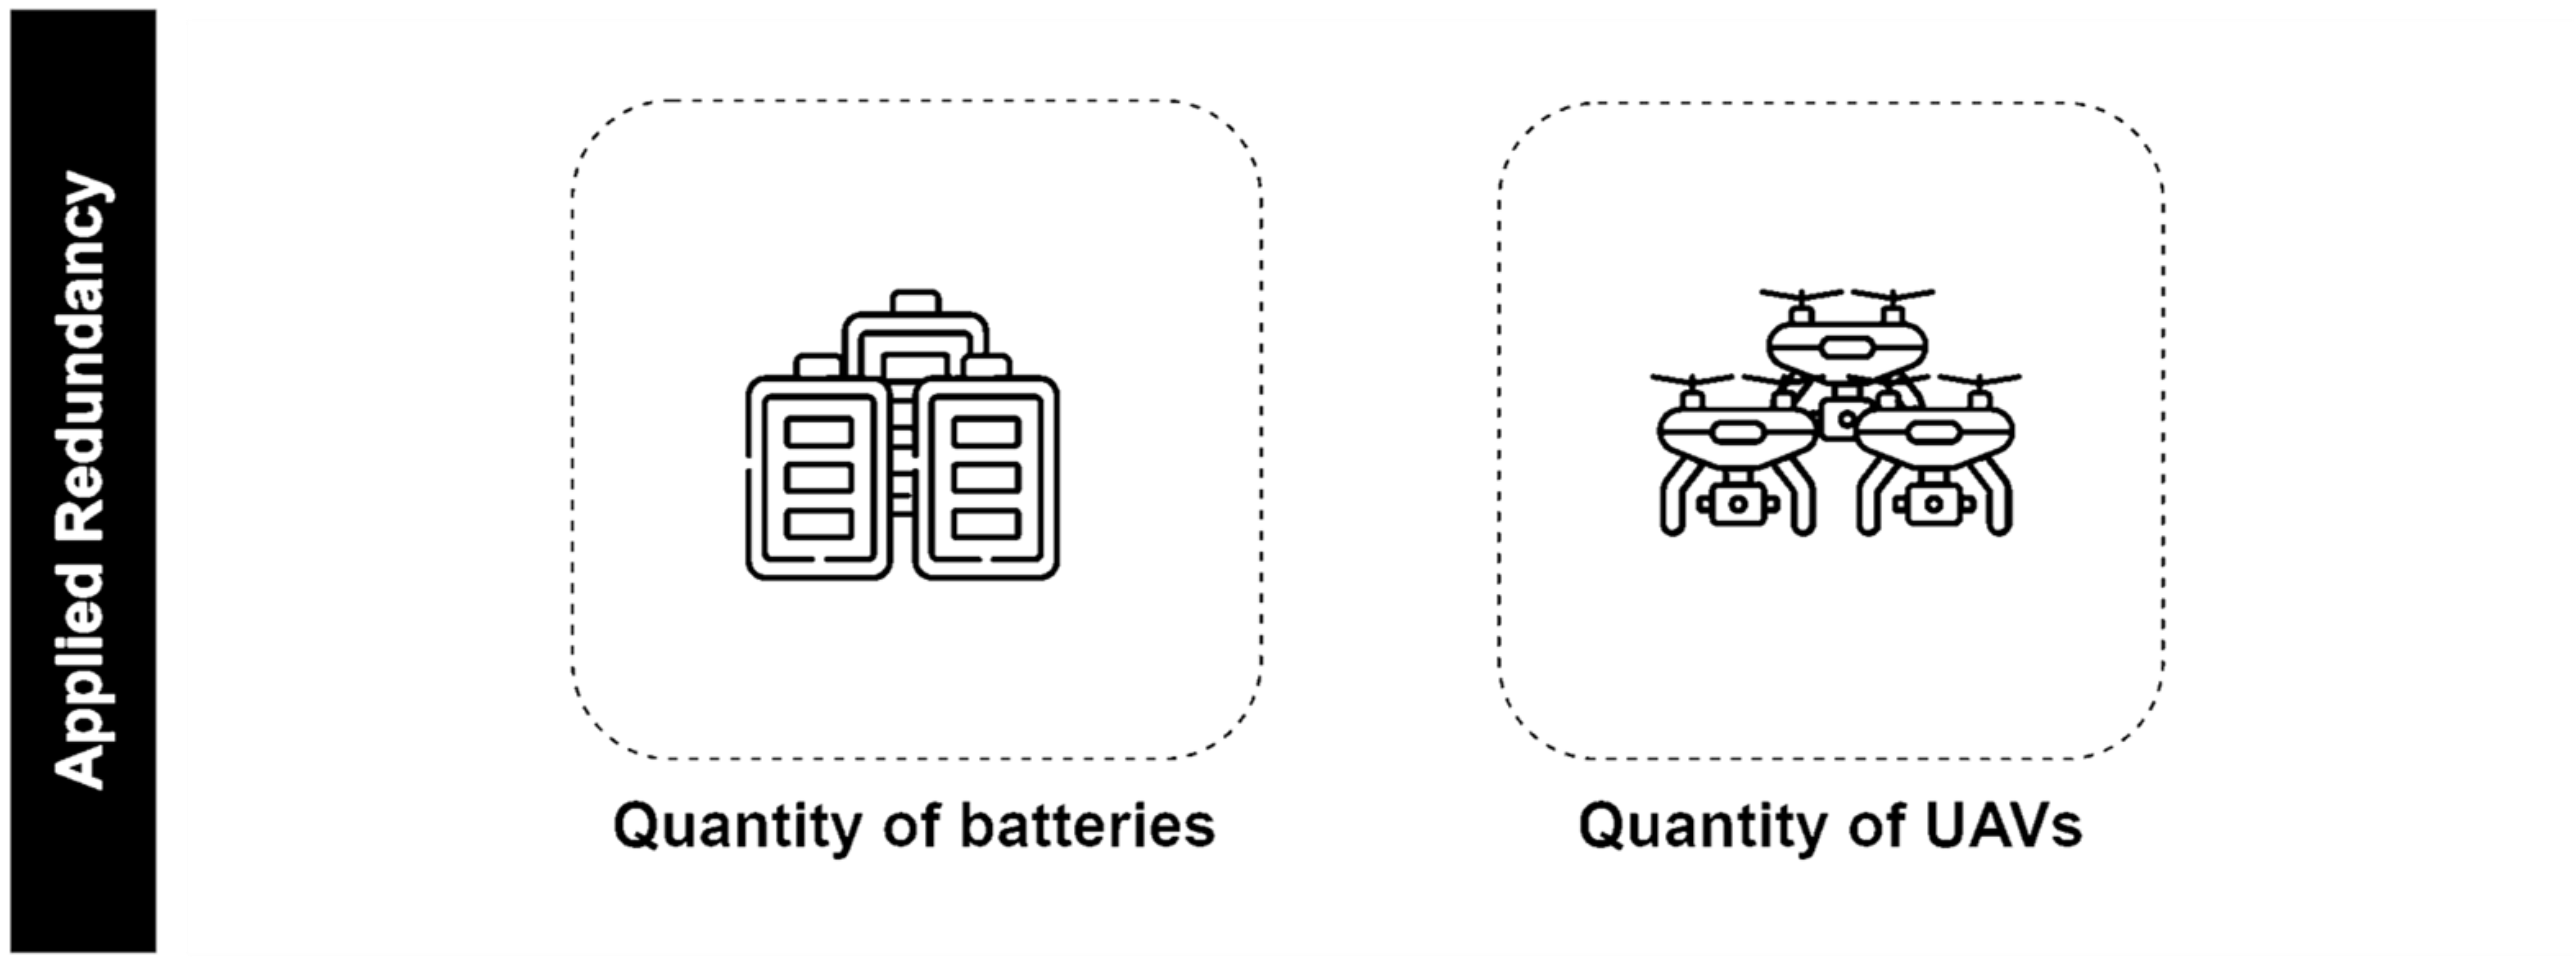
\includegraphics[scale=0.22]{img/operating_model_study_02.png}}
\caption{Applied Redundancy.}
\label{fig:case_study_02}
\end{figure}

In this Case Study \#2, we evaluate the impact of using N UAVs and battery redundancy on system availability (Fig. \ref{fig:case_study_02}). To represent systems with redundancy mechanisms using continuous-time Markov chain models (CTMC) or even analytical models with equations, we would have to face state explosion, which makes it challenging to understand CTMC and manually calculate the generated analytical equations.

A stochastic Petri net (SPN) model facilitates systems modeling with redundancy mechanisms, such as the UAV flight system availability model. SPNs are numerical models evaluated by software simulation. We will use the Mercury tool \citep{maciel2017mercury} to evaluate the model for this study. The input parameters of the SPNs are given by times (MTTs). For example, Table \ref{tab:basic_spn_parameter_values} shows the baseline system MTTs composed of the same values as in Case Study 1 in time format.

\begin{table}[htbp]
\caption{Parameter values for the SPN model}
\begin{center}
\begin{tabular}{c|c}
\hline
\textbf{\textit{Parameter}} & \textbf{\textit{Value (hours)}} \\
\hline
\hline
 MTTFD & 5000\\
 MTTRD & 2\\
 MTTBD & 0.5 \\ 
 MTTBC & 2 \\
 MTTDS & 0.166666667 \\
 NB & 1 \\
 ND & 1 \\
\hline
\end{tabular}
\label{tab:basic_spn_parameter_values}
\end{center}
\end{table}


Figure \ref{fig:basic_spn_sa_battery} shows the evolution of the system's general availability only with the application of redundancy in the battery component (NB). We achieved 0.85\% availability using eight ready-to-use spare batteries. With the value of spare batteries fixed at 8, we vary the value of spare drones (ND) and get the availability of nine (0.90\%) from four spare drones (Figure \ref{fig:basic_spn_sa_uav}). However, we cannot achieve availability with numbers of nines greater than 0.9\% just by adding redundancy mechanisms or improving the timing of baseline system components.

\begin{figure}[htbp]
\centerline{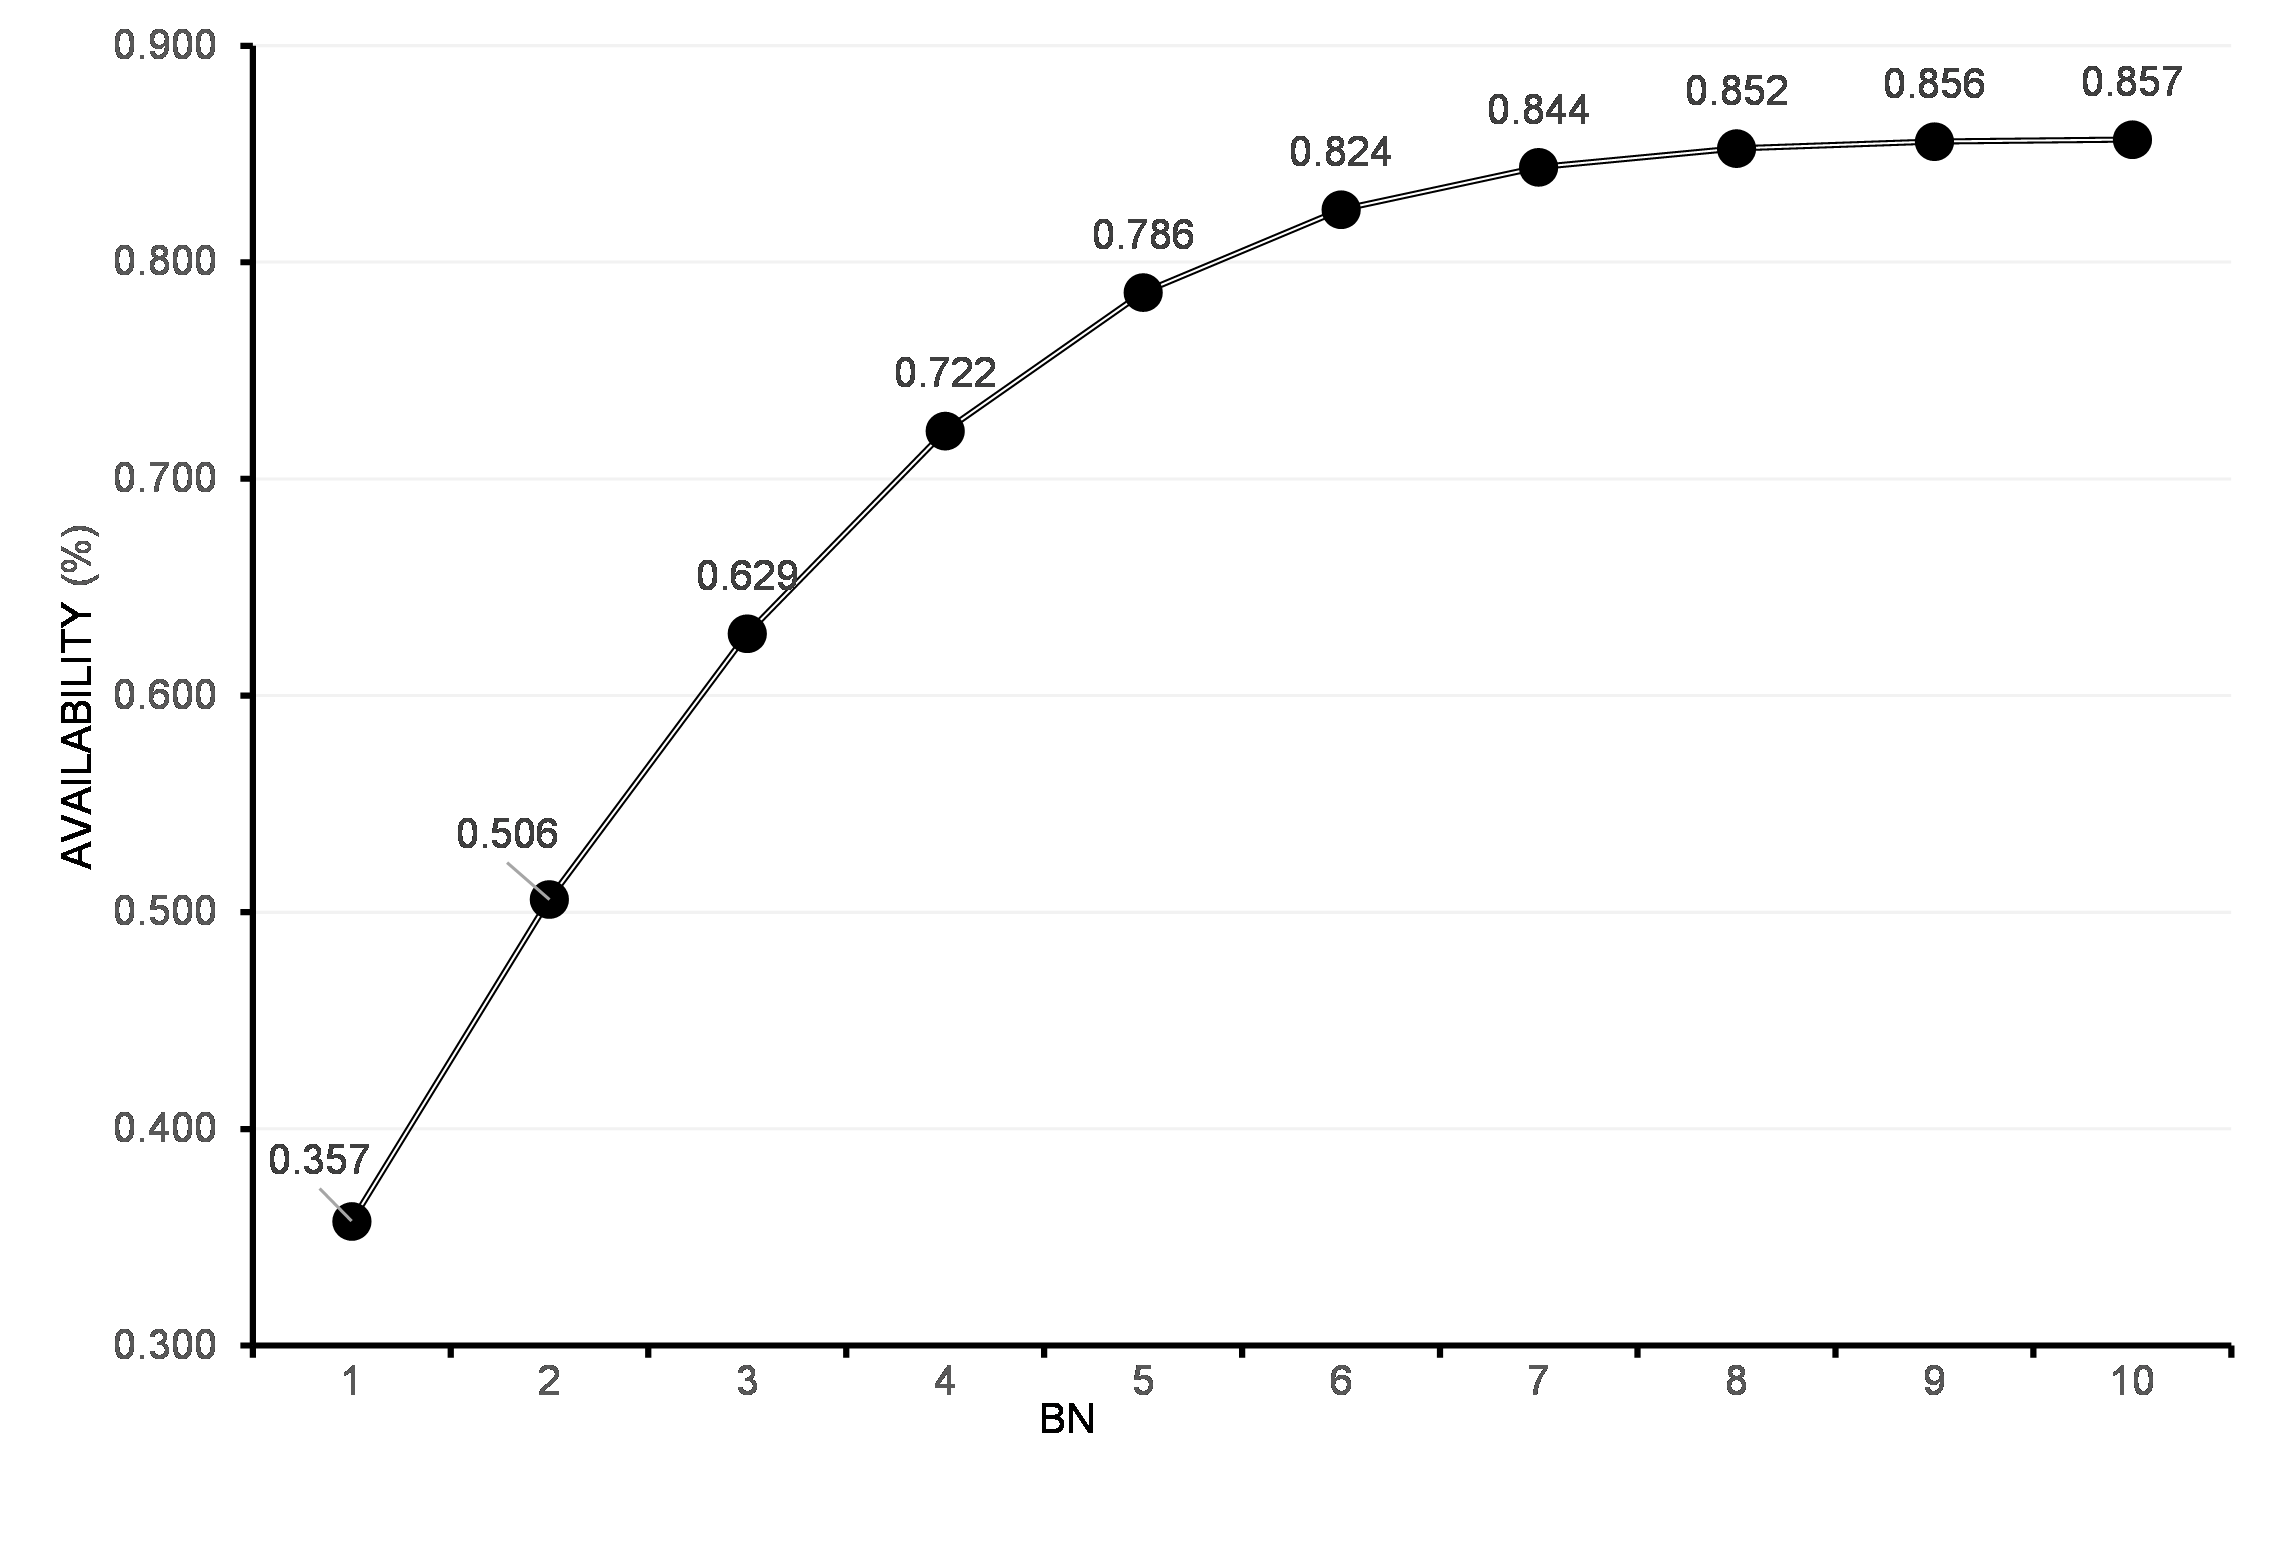
\includegraphics[scale=0.45]{img/exps/SA_006.png}}
\caption{Availability by the number of batteries with basic operating mode MTT parameters}
\label{fig:basic_spn_sa_battery}
\end{figure}

\begin{figure}[htbp]
\centerline{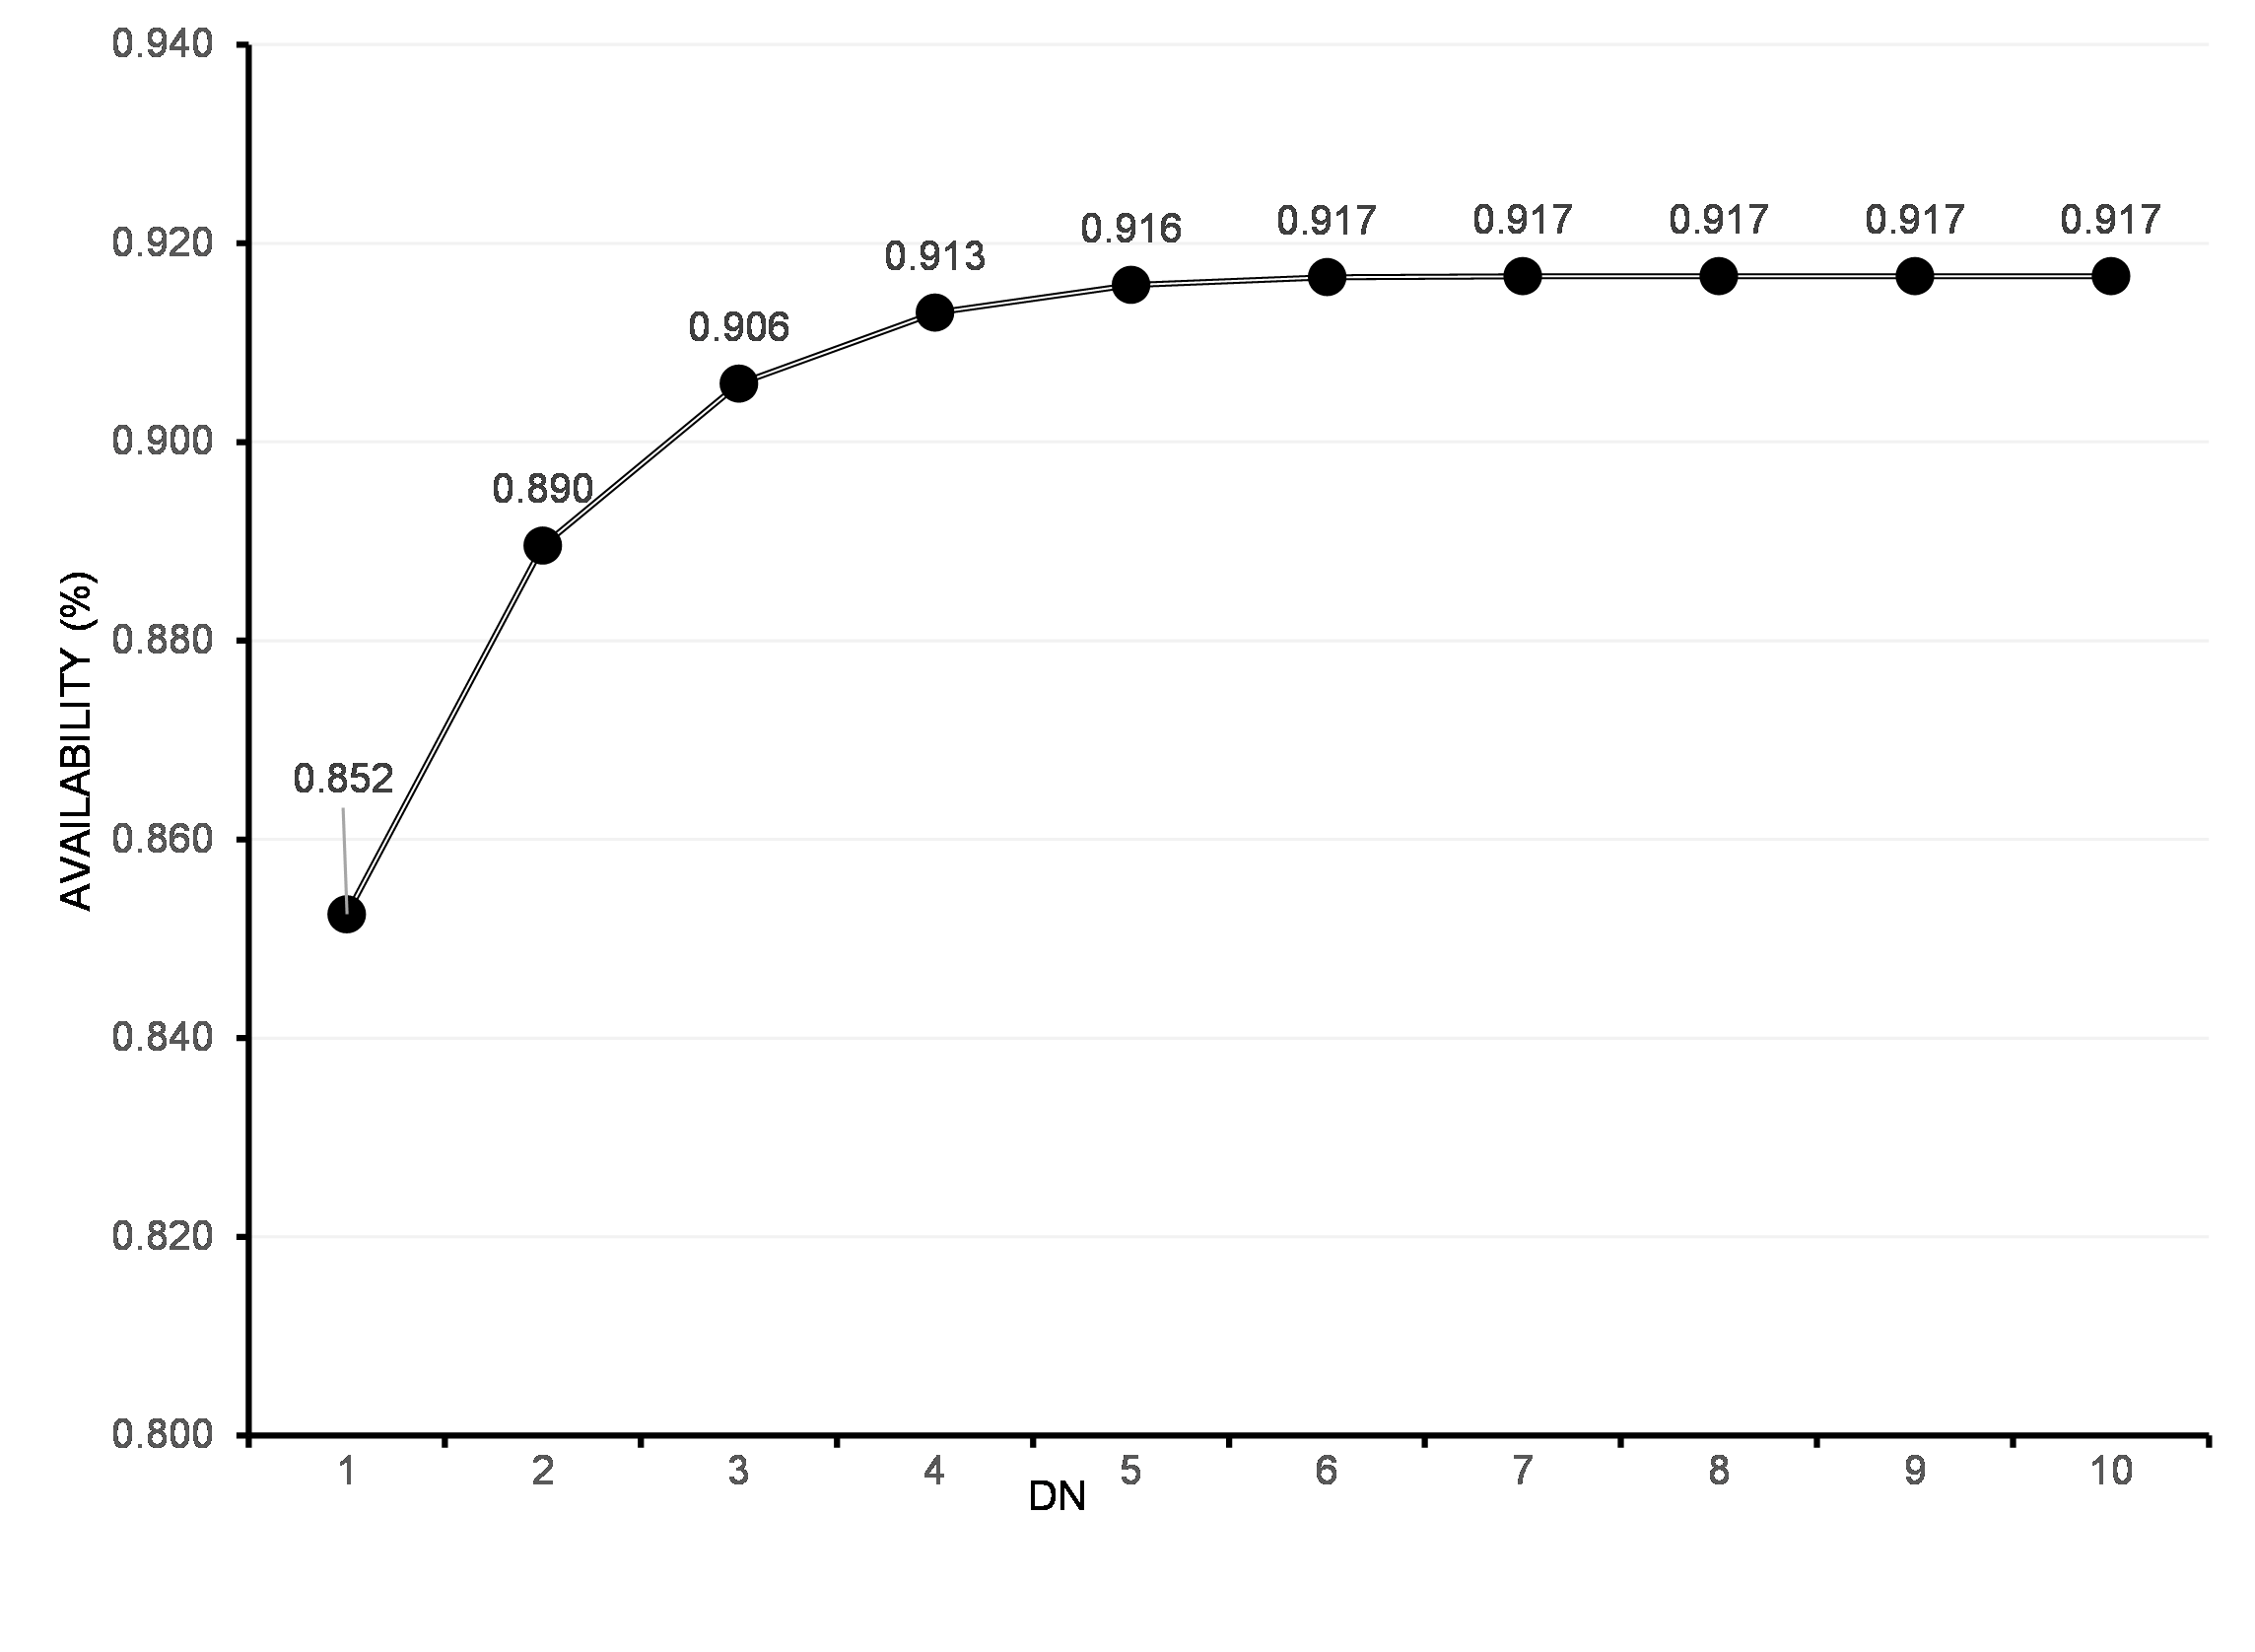
\includegraphics[scale=0.45]{img/exps/SA_003.png}}
\caption{Availability by number of UAVs with basic operating mode MTT parameters}
\label{fig:basic_spn_sa_uav}
\end{figure}


\subsection{Case Study \#3}
\label{sec:case_studies_sub03}

This third case study combines the previous two. Redundancy variations of the spare UAV components will be evaluated using improved UAV load, unload, and switchover times parameters from Case Study \#1 to achieve higher availability than the first two case studies. The enhanced time values used as input are defined in Table \ref{tab:spn_parameter_values}.

\begin{table}[htbp]
\caption{Improved parameter values for the SPN model}
\begin{center}
\begin{tabular}{c|c}
\hline
\textbf{\textit{Parameter}} & \textbf{\textit{Value (hours)}} \\
\hline
\hline
 MTTFD & 5000\\
 MTTRD & 2\\
 MTTBD & 2 \\ 
 MTTBC & 0.5 \\
 MTTDS & 0.016666667 \\
 NB & 1 \\
 ND & 1 \\
\hline
\end{tabular}
\label{tab:spn_parameter_values}
\end{center}
\end{table}


At first, it is possible to obtain availability with the number of nines equal to 2 (0.993\%) only with the addition of an extra battery (Figure \ref{fig:spn_sa_battery}), with initial availability of improved study parameters from case 1 of 0.97\%. Finally, Figure \ref{fig:spn_sa_uav} shows the availability of 0.999\% using only 5 UAVs and two backup batteries with timing improvements.

\begin{figure}[htbp]
\centerline{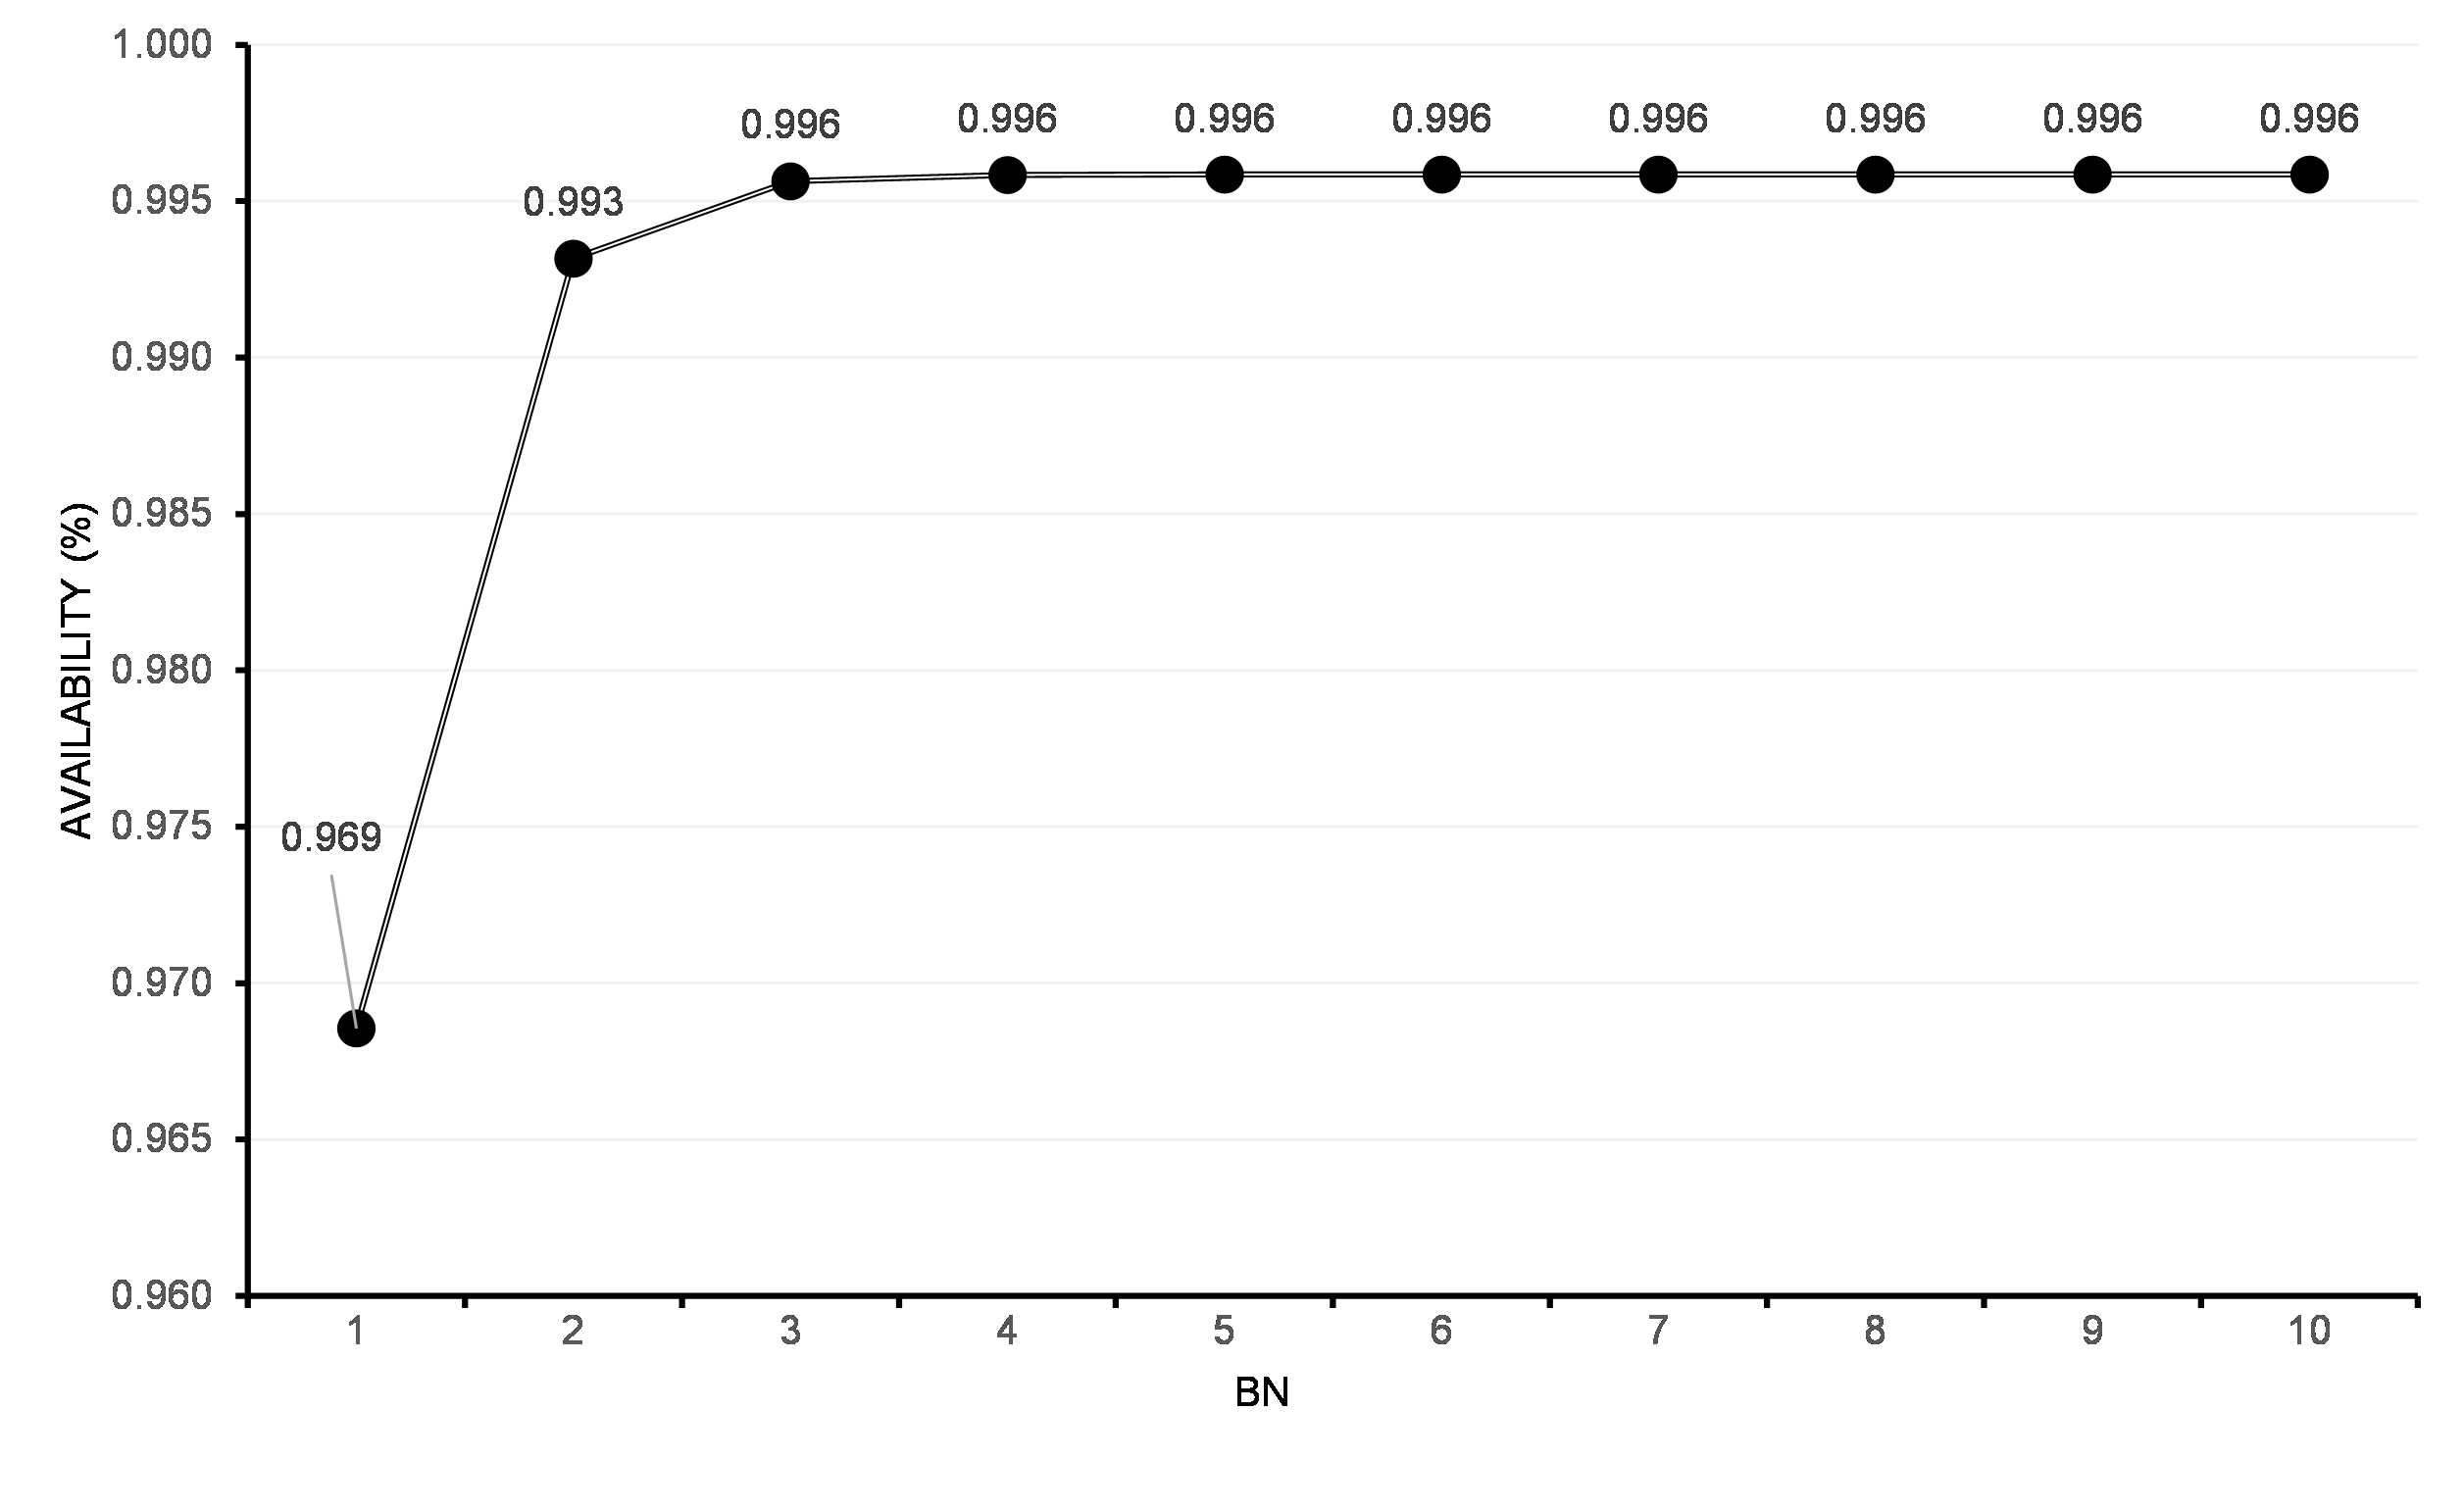
\includegraphics[scale=0.4]{img/exps/SA_005.png}}
\caption{Availability by the number of batteries with improved MTT parameters}
\label{fig:spn_sa_battery}
\end{figure}

\begin{figure}[htbp]
\centerline{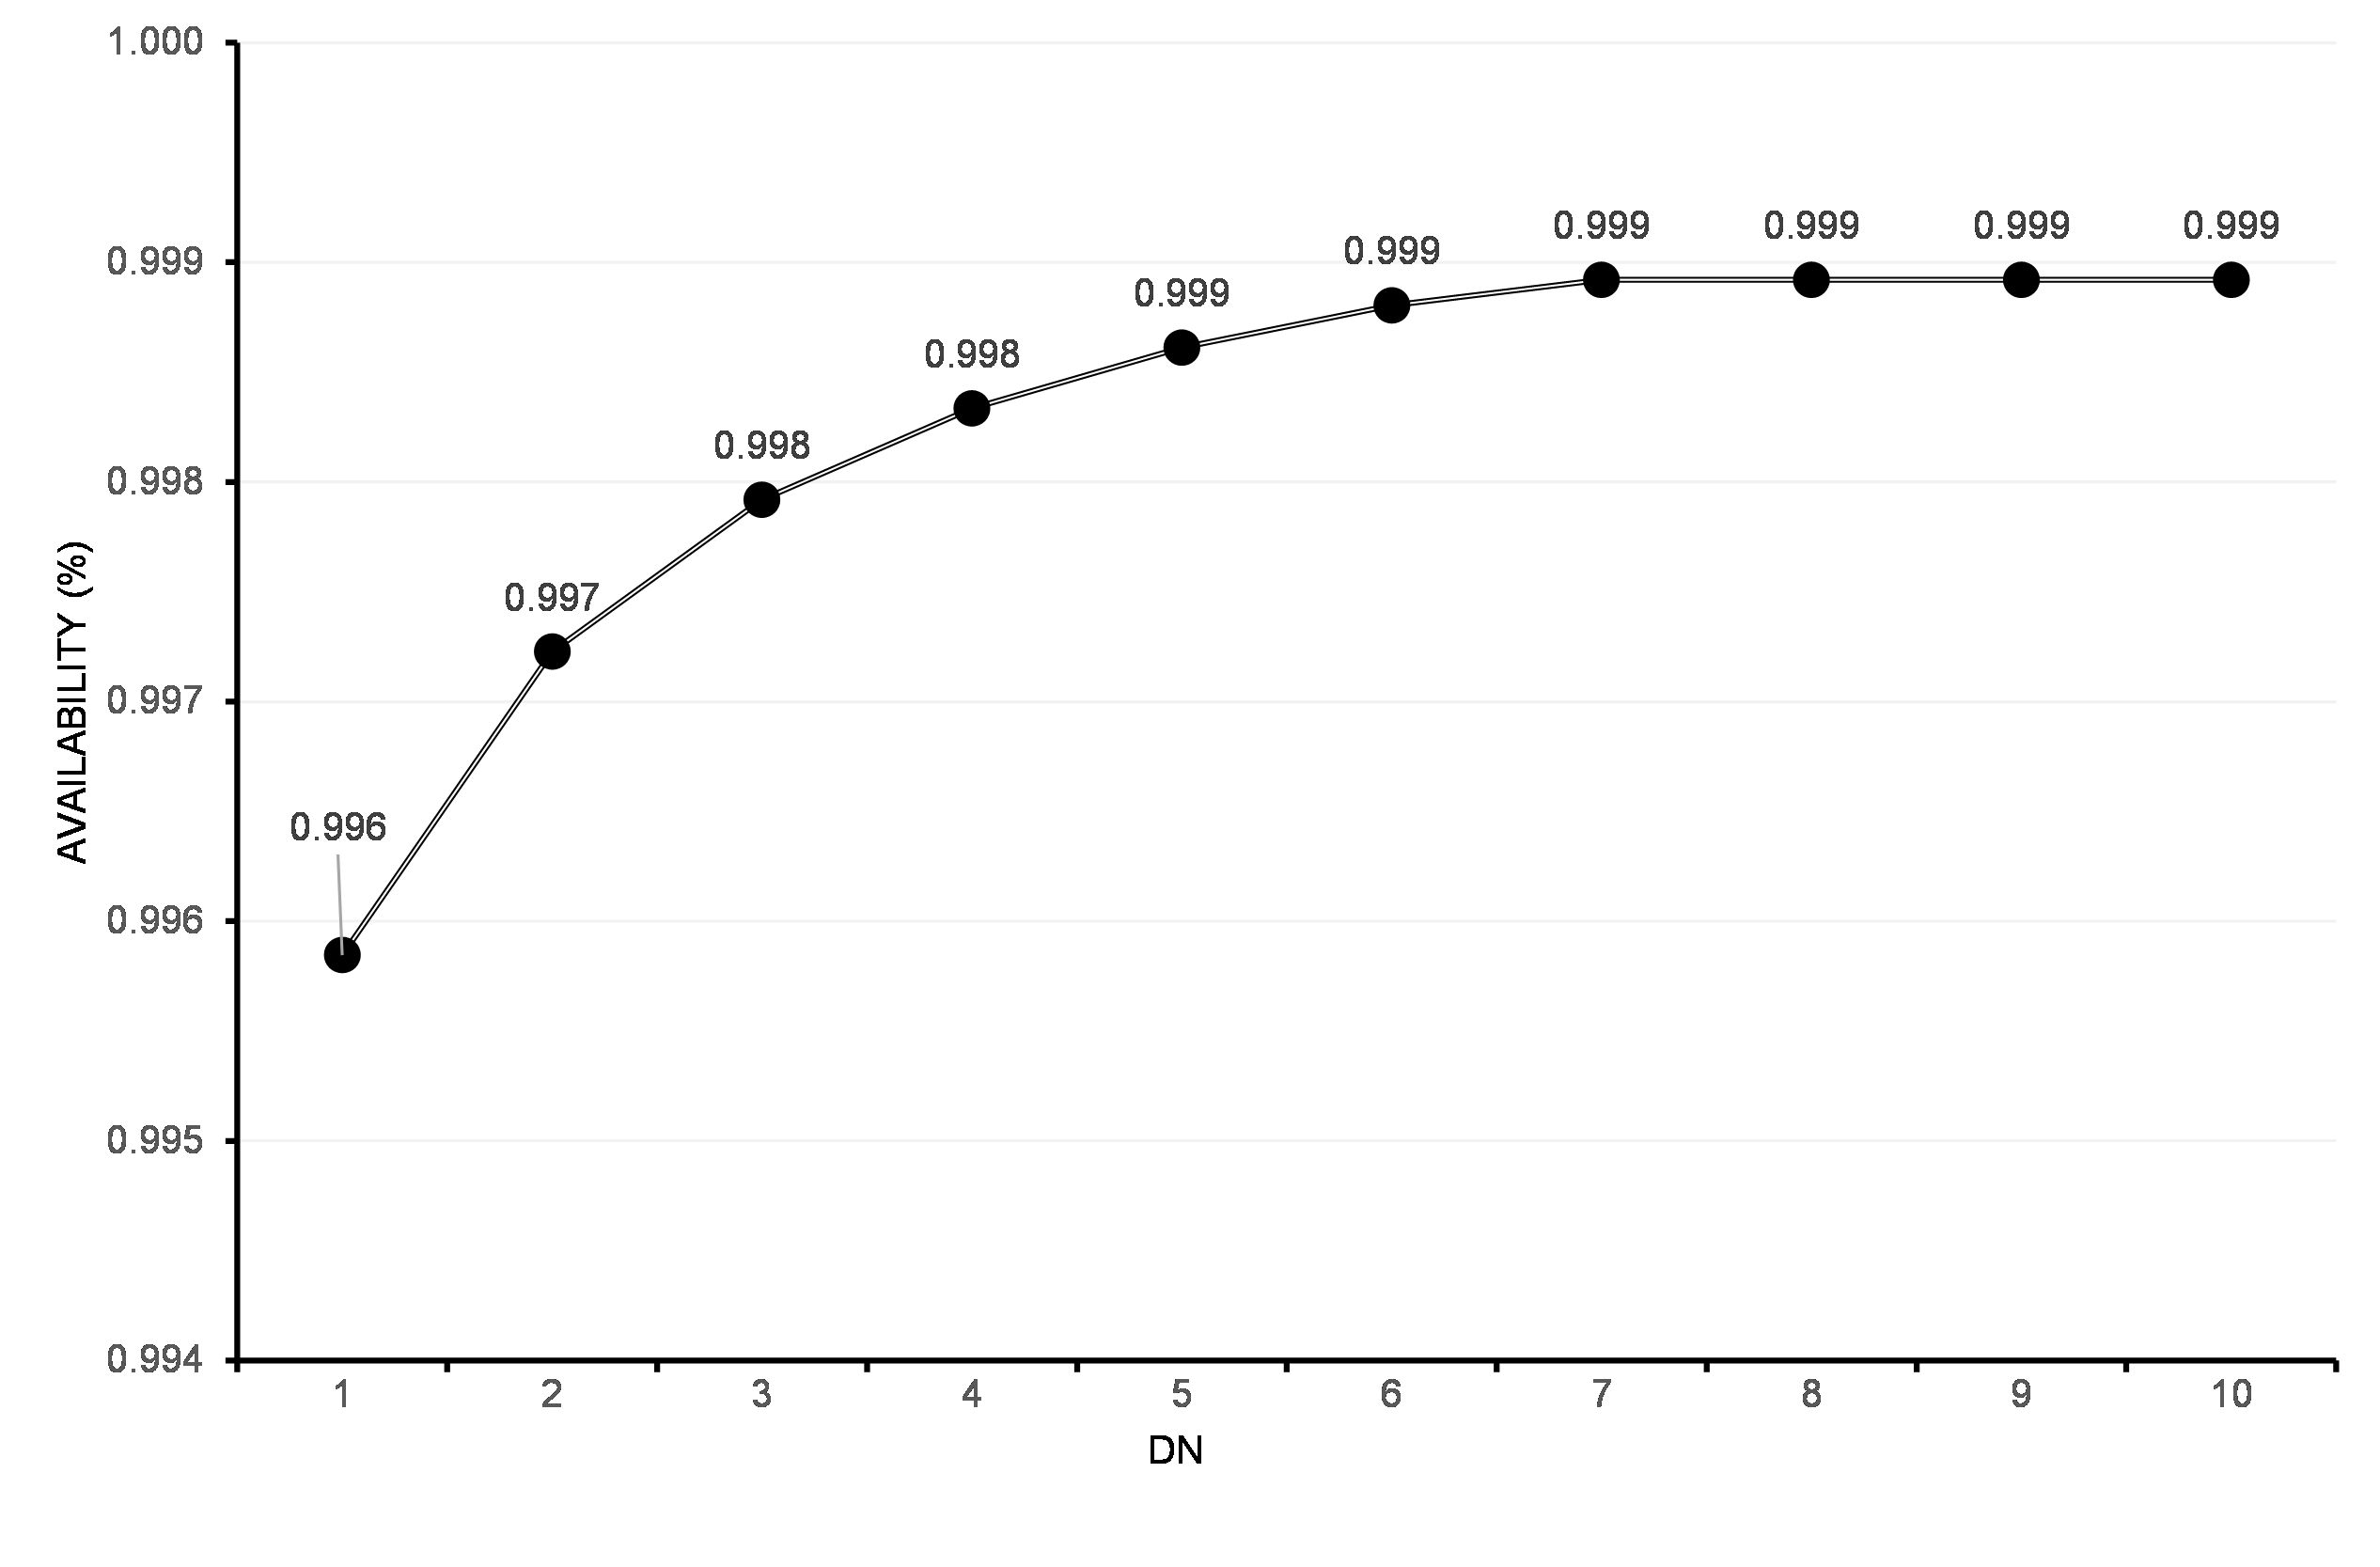
\includegraphics[scale=0.4]{img/exps/SA_004.png}}
\caption{Availability by number of UAVs with improved MTT parameters}
\label{fig:spn_sa_uav}
\end{figure}

The use of fewer UAVs and spare batteries compared to the previous study may represent a considerable discount on the final budget for a system with these characteristics.


%-----------------------------------------------------------------------------------------------
\section{Conclusions and future work}
\label{sec:conclusions}

This work proposes two models for evaluating the availability of critical monitoring systems implemented in UAV devices. In three case studies, an assessment of the system's availability has been carried out, given the improvements made and the models used. 

The first case study varies baseline system time parameters, symbolizing component improvements. As a result, the improvements had limited availability of 0.97\%. In the second case study, using redundancy mechanisms and a Petri net model with the same baseline, the availability improvement was limited to 0.91\% with eight batteries and six spare UAVs. Finally, in the last case study, there was a significant improvement in availability, benefiting from improvements in the components with the joint use of redundancy mechanisms, which allowed an overall availability of the system of the order of three nines, 0.999\%.

In future work, we intend to evaluate the cost vs. availability metrics of the case studies performed and compare this type of system implemented in the cloud, fog, and edge computing paradigms.

%-----------------------------------------------------------------------------------------------
\section*{Acknowledgment}
\label{sec:acknowledgment}
The authors would like to thank the Brazilian government for financial support through the Fundação de Amparo a Ciência e Tecnologia de Pernambuco (FACEPE), Modeling Distributed and Concurrent Systems (MoDCS) group for helping to improve this research.

%-----------------------------------------------------------------------------------------------
\bibliographystyle{plainnat}
\bibliography{references}


\end{document}